\documentclass[a4paper, 11pt, twoside, titlepage]{book}
% Set up page layout
\usepackage[a4paper]{geometry}
\usepackage{fancyhdr}
% Set up hyphenation, etc.
\usepackage[british]{babel}
% Set up images
\usepackage{pstricks,pst-node,pst-text,pst-3d,pst-eucl}
\usepackage{psfrag}
\usepackage{import}
\usepackage{graphicx}
\usepackage{subfigure}
\usepackage[figuresright]{rotating}
%\usepackage{flafter}
% Set up fonts
\usepackage{charter}
\usepackage{amssymb,amstext,amsfonts} %% ... with default font
\usepackage{amsmath}
\usepackage{mathrsfs}
%\usepackage{txfonts}
% Colouring
\usepackage{xcolor}
\definecolor{vermilion}{rgb}{0.80,0.40,}
\definecolor{blueishgreen}{rgb}{0,0.60,0.50}
\definecolor{skyblue}{rgb}{0.35,0.70,0.90}

% Set up lists and tables
\usepackage{listings}
\usepackage{enumitem}
\setlist{itemsep=0pt}
\usepackage{booktabs, longtable, dcolumn,multirow}
\usepackage{array}
\usepackage{ragged2e}
\newcolumntype{P}[1]{>{\RaggedRight\hspace{0pt}}p{#1}}
\usepackage[labelfont=bf,labelsep=space,hypcap]{caption}
\renewcommand{\captionfont}{\small}
\usepackage[caption2]{ccaption}
%\usepackage{tikz}
%\usetikzlibrary{shapes,arrows}
% More fonts
\usepackage[T1]{fontenc}
\usepackage{lmodern}
\renewcommand{\sfdefault}{lmss}
\renewcommand{\ttdefault}{lmtt}
\usepackage{microtype}
\usepackage[latin9]{inputenc}
\usepackage[11pt]{moresize}
%\usepackage{fixmath}
\usepackage{ upgreek }
% Special symbols
\usepackage{braket}
\usepackage{slashed}
% Set up page indexing, bib fomatting, etc.
\usepackage{afterpage}
\usepackage{appendix}
%\usepackage{paralist}
%\usepackage[linktocpage,bookmarksnumbered,breaklinks,pdfhighlight=/P,citebordercolor=blueishgreen,urlbordercolor=skyblue,linkbordercolor=vermilion]{hyperref}
\usepackage[authoryear]{natbib}
\usepackage[linktocpage,bookmarksnumbered,pdfauthor={Christopher P.L. Berry},pdftitle={Exploring Gravity},pdfkeywords={Ph.D. Dissertation}]{hyperref}            
\usepackage{bookmark}
\usepackage{etoolbox}
% Only link on year
\makeatletter

% Patch case where name and year are separated by aysep
\patchcmd{\NAT@citex}
  {\@citea\NAT@hyper@{%
     \NAT@nmfmt{\NAT@nm}%
     \hyper@natlinkbreak{\NAT@aysep\NAT@spacechar}{\@citeb\@extra@b@citeb}%
     \NAT@date}}
  {\@citea\NAT@nmfmt{\NAT@nm}%
   \NAT@aysep\NAT@spacechar\NAT@hyper@{\NAT@date}}{}{}

% Patch case where name and year are separated by opening bracket
\patchcmd{\NAT@citex}
  {\@citea\NAT@hyper@{%
     \NAT@nmfmt{\NAT@nm}%
     \hyper@natlinkbreak{\NAT@spacechar\NAT@@open\if*#1*\else#1\NAT@spacechar\fi}%
       {\@citeb\@extra@b@citeb}%
     \NAT@date}}
  {\@citea\NAT@nmfmt{\NAT@nm}%
   \NAT@spacechar\NAT@@open\if*#1*\else#1\NAT@spacechar\fi\NAT@hyper@{\NAT@date}}
  {}{}

\makeatother

\renewcommand{\bibfont}{\footnotesize}
\addto{\captionsbritish}{\renewcommand{\bibname}{{R\lowercase{eferences}}}}
%\renewcommand{\refname}{{R\lowercase{eferences}}}
\setlength{\bibhang}{0pt} 
%\setlength{\bibsep}{0.5pt} % 1 linestretch
\setlength{\bibsep}{0pt} % 1.3 linestretch
\addto{\captionsbritish}{\renewcommand{\contentsname}{{C\lowercase{ontents}}}}

%\usepackage{fourier-orns}
  
% Set page layout  
\headheight 13.6pt
% For 10pt text
%\headsep 0.6\baselineskip
%\footskip 2\baselineskip
%\textheight = 55\baselineskip
% For 11pt text
\topmargin -0.4cm
\headsep 0.6\baselineskip
\footskip 2\baselineskip
\textheight = 50.1\baselineskip

\allowdisplaybreaks

% Set numbering depth
\setcounter{secnumdepth}{5}

\def\today{\number\day\space\ifcase\month\or January\or February\or March\or April\or May\or June\or July\or August\or September\or October\or November\or December\fi\space\number\year}

% Custom commands
\newcommand{\eqnref}[1]{equation (\ref{eq:#1})}
\newcommand{\Eqnref}[1]{Equation (\ref{eq:#1})}
\newcommand{\secref}[1]{section \ref{sec:#1}}
\newcommand{\Secref}[1]{Section \ref{sec:#1}}
\newcommand{\chapref}[1]{chapter \ref{ch:#1}}
\newcommand{\Chapref}[1]{Chapter \ref{ch:#1}}
\newcommand{\partref}[1]{part \ref{pt:#1}}
\newcommand{\Partref}[1]{Part \ref{pt:#1}}
\newcommand{\apref}[1]{appendix \ref{ap:#1}}
\newcommand{\Apref}[1]{Appendix \ref{ap:#1}}
\newcommand{\tabref}[1]{table \ref{tab:#1}}
\newcommand{\Tabref}[1]{Table \ref{tab:#1}}
\newcommand{\figref}[1]{figure \ref{fig:#1}}
\newcommand{\Figref}[1]{Figure \ref{fig:#1}}

\newcommand{\units}[1]{\ensuremath{~\mathrm{#1}}}

\newcommand{\sub}[1]{\ensuremath{_\mathrm{#1}}}
\newcommand{\super}[1]{\ensuremath{^\mathrm{#1}}}

\begin{document}

\bibpunct{(}{)}{;}{a}{}{,\,}

\makeatletter
\pagestyle{fancy}
\renewcommand{\sectionmark}[1]{\markright{\thesection\ #1}}
\fancyhf{}
\fancyhead[LE]{Summative assessment}
\fancyhead[RE]{Christopher Berry}
\fancyhead[LO]{FLTHE}
\fancyhead[RO]{\rightmark}
%\fancyhead[RO]{}
\fancyfoot{}
\renewcommand{\footrulewidth}{0.1ex}
\fancyfoot[LO]{\today}
%\fancyfoot[LO]{21st August 2013}
\fancyfoot[RE]{University of Birmingham}
\fancyfoot[RO, LE]{\thepage}
\fancypagestyle{plain}{
\fancyhf{}
\renewcommand{\headrulewidth}{0pt}
\fancyfoot{}
\renewcommand{\footrulewidth}{0.1ex}
\fancyfoot[LO]{\today}
\fancyfoot[RE]{University of Birmingham}
\fancyfoot[RO, LE]{\thepage}}
\makeatother

\frontmatter

\title{{\large\textsc{Foundation of Learning \& Teaching in Higher Education}}\\
\vspace{-5mm}\hrulefill\\
{\Huge\textsc{Tutoring Second-Year Physics\\\& Key Skills}}\\
\vspace{-2mm}\hrulefill\\
\vspace{-2mm}{\large\textsc{Postgraduate Certificate in Academic Practice}}}

\author{{\Large{}Christopher Berry}\\
\vspace{1mm}\href{mailto:cplb@star.sr.bham.ac.uk}{cplb@star.sr.bham.ac.uk}\\
\vspace{1mm}School of Physics \& Astronomy}

\date{\today} 

\maketitle

\tableofcontents

\mainmatter

\chapter{Overview}

In this work we examine the small-group teaching of second-year physics undergraduates. This teaching takes the form of regular tutorials. The role of small-group tutorials (SGTs) within physics is introduced in \chapref{intro}.\footnote{In the context of teaching physics, we consider a small group to be one consisting of 2--6 students, which follows \citet[chapter 1]{Jaques2007}. My own groups range in size between 2 and 5 students.} Here, I reflect upon my own educational experiences as well as research on teaching and learning \citep{McCarthy2008}. One of the components of tutorials is the teaching of key skills: compiling a curriculum vit\ae{} (CV), giving a presentation and writing an essay. These transferable skills are valuable assets when the students graduate and seek employment \citep{Pike2015}. Teaching these communication skills is different from the more familiar teaching of subject material and so I have chosen to examine my practices in more detail, concentrating on essay writing. In \chapref{essay} I discuss a plan for this teaching, I introduce a new elements to my delivery, a formative essay designed to give feedback \citep[feedforward;][]{Bloxham2015} and practice, and blog posts that can be referred to outside of tutorial.\footnote{The posts can be read at \url{http://cplberry.com/tag/writing/}.} In \chapref{conc}, I evaluate their impact. In the process of this, I draw upon feedback from students (\apref{student}) and peers (\apref{peer}), my own training (e.g., \apref{Scriptoria}), and the final marks (\apref{marks}). I find that the formative essay has a small positive effect on the achievement of my students, but this impact could potentially be improved by adapting its format; as might be expected, the students' motivation and proficiency remain the dominant predictors of their essay-writing ability \citep{Ketteridge2015}.


\chapter{Introduction to tutoring physics}\label{ch:intro}

In this chapter we discuss the teaching and learning of physics with particular reference to my experiences. We learn from our own experiences, repeating things that have gone well, and avoiding those that led to failure \citep[chapter 2]{Skinner1954,Kolb1984}. When reflecting upon our own teaching, we must consider how our own perception is influenced by our own experience, and how our students may not share the same view;\footnote{The Johari window gives a simple way of visualising how one's own experience does not overlap with others', but one's outlook can be expanded through feedback \citep{Luft1961}. Sharing experiences (exposing one's own knowledge) with others can be considered an aspect of teaching \citep[cf.][chapter 7]{Ramsden1992}.} hence, we begin with a brief summary of my personal development to date in \secref{teach-n-learn}. We continue from here by introducing core components of studying physics (\secref{physics}), before expanding upon small-group teaching (\secref{small}) which has been a primary component of both my learning and teaching experience. Building upon the ideas of learning in a small group, my experiences of learning through peer collaboration are discussed in \secref{peer}. The chapter concludes with a critique of how I have assimilated aspects of my own student experience into my approach to teaching.

\section{Teaching \& learning}\label{sec:teach-n-learn}

My own teaching style reflects how I learnt as I attempt to emulate the experiences that were most educational for me. Given that I was both sufficiently academically able and interested in my subject to continue to hold a university research position, it may be assumed that I do not reflect the average student. Therefore, while my personal experience is a sensible starting point, it is vital to remember that others may have different preferences \citep[chapter 5]{Ramsden1992} and those who need the most support will be those who find the subject more difficult than I did. To try to understand other perspectives and broaden my outlook, it is necessary to seek feedback (see appendices \ref{ap:student} and \ref{ap:peer}) and research studies of educational practices (discussed throughout).

I read Natural Sciences at the University of Cambridge as an undergraduate, specialising in Experimental and Theoretical Physics, before continuing to complete a Ph.D.\ in Astronomy. During my postgraduate study I began supervising: tutoring small groups (2--3 students), with teaching focused on weekly (formative) problem sets. These had been an integral part of my undergraduate study, hence I was familiar with their function and form. Following completion of my doctorate, I have moved to the University of Birmingham, where I now tutor: small-group (3--5 students) teaching similar to supervising, except that problems also play a summative role. At both Cambridge and Birmingham, I have taught second-year physics for these SGTs.

In the last academic year, I have continued my personal development by lecturing a short, optional course to a mix of fourth-year undergraduates and postgraduate students.\footnote{The course was approximately $52\%$ undergraduates, $34\%$ postgraduates and $14\%$ interested staff.} Lecturing will not be discussed in detail in this work, but there are many parallels between SGTs and lectures, such as needing to explain clearly; maintain an environment suitable for learning; check students' understanding and progress; plan material to deliver and do so at good pace (within a fixed time); engage students in discussions and interest them in their studies, and seek feedback from students (\citealt[chapter 3]{Brown1988}; cf.\ \citealt[chapter 6]{Ramsden1992}).\footnote{Tutorials can become too much like lectures \citep[chapter 9]{Ramsden1992}; in a study of SGTs in British universities, \citet[quoted in \citealt{Brown1988}, chapter 4]{Luker1987} found that between $7\%$ and $70\%$ of the time is spent by the tutor lecturing.} I found that my experience with SGTs made it more natural for me to engage with the class and have them work through problems, which proved popular. I was surprised how difficult it was to judge how long it would take to cover a particular topic. I am used to going through problems and explaining concepts in tutorials, and keeping to an hour time-slot; however, extending this to a lecture where a single narrative, explained such that a large group can keep up, must be contained within a hour was challenging. This has made me more conscious of how I allocate time in tutorials, and in particular that I leave time for a summary at the end to recap what we have discussed.\footnote{The usefulness of an ending summary was highlighted through my experience of peer observations (both reflecting on feedback on my tutorials and while observing the lecturing of another) discussed in \apref{peer}.}

\section{Studying physics}\label{sec:physics}

Physics is a broad subject covering the fundamental behaviour of the Universe and its components. It is familiar to most as it is introduced at school level: its teaching follows a spiral curriculum, periodically returning to previously-taught topics to cover them in ever-expanding detail \citep{Bruner1960}. The main jump from school to university physics is in the use of mathematics. Applying mathematical formalism to describe and solve physical problems is the greatest threshold concept \citep{Meyer2003} faced by those wishing to become conversant with physics \citep{Wigner1960}.

My experience of university-level physics teaching has been traditional \citep[cf.][]{Iannone2015}. Concepts and theories are introduced in lectures. These ideas are reinforced through problem sets that also encourage mathematical fluency and independent learning \citep{Pike2015}. At least some of these problems are assessed to provide students with feedforward information \citep{Bloxham2015}. SGTs or examples classes give students the opportunity to discuss the problems and their solutions, as well as other elements of the syllabus.\footnote{This may fulfil the role of inverted classrooms, where students prepare outside of class and then work through problems under the guidance of a tutor in class, employed elsewhere \citep{Lage2000}.} Practical work is done in labs; experiments may complement topics covered in lectures, for example measuring refraction during a course on electromagnetism; be of equal importance as lectures for teaching ideas, for example in a course on electronics, or motivate material covered in lectures, for example error analysis \citep{Hanif2009}. Assessment is dominated by summative closed-book examinations at the end of the courses.\footnote{The situation may be comparable to that in mathematics where traditional closed-book examinations are favoured \citep{Iannone2014}, as both subjects require similar (mathematical) problem solving and the correctness of solutions is not subjective.} I have found completing problem sets to best encourage deep learning \citep{Marton1976,Marton1976a}: good understanding is required to fully solve a question and, since problems are done outside of class, there is sufficient time to review and assimilate new ideas.\footnote{Even if a student takes an achieving strategy \citep[chapter 2]{Biggs1987} and only invests time in understanding the topics directly probed by the given questions, a dense covering of the syllabus by problems sets should ensure a comprehensive understanding of the majority of the material.}

Problem sets are of paramount importance, both for teaching subject material and key skills such as problem solving and mathematical proficiency. Extracting the most from them relies on the student being motivated to put in the necessary effort: those who work harder shall learn more \citep{Gibbs2015}. This is difficult to externally inspire \citep[cf.][]{Ryan2000}, especially since a student taking a surface-learning approach is more likely to find problems tedious and unprofitable, potentially pushing them further away from engaging with the material \citep[chapter 4]{Ramsden1992}. Consequently, we shall instead focus on how problem sets are supported, which is primarily through SGTs.

\section{Small-group teaching}\label{sec:small}

Supervisions at Cambridge involve either an academic or a Ph.D.\ student meeting regularly with a group of students. The small group size allows for sessions to be tailored to the individual needs of the students and for each student to be involved in discussions.\footnote{Groups of only one student are usually avoided as this could be intimidating for the student. Furthermore, having an additional student provides some respite to think while the other is being questioned. The lone student would also miss out on the opportunity to hear the opinions of a peer.} Supervisions are generally structured around the problems, with the students given opportunity to ask about other areas of the course they were unsure of (or interested in); any spare time is used to discuss additional topics (perhaps the research of the supervisor). The supervision system is designed to encourage students to stay on top of their work and to provide them with the necessary support when this is difficult; the overall effect is to promote deep learning \citep[case study 14.1]{Gibbs2015}.

Tutorials in Birmingham are of a similar nature to supervisions. They differ in group size, which does not afford as intensive attention to individual students, and also in the amount of contact time. In second year, Cambridge's Natural Sciences undergraduates would have one hour per week per course (three hours per week in total), while Birmingham's Physics undergraduates have a single hour per week for all their courses.\footnote{The difference in teaching time is slightly ameliorated by the marginally longer teaching year in Birmingham: 22 weeks compared to 19.} While the tutorial system might not match supervisions in Cambridge, they still provide a great opportunity for students to engage with and ask questions of a member of research staff, an opportunity that is not present as part of all physics courses.\footnote{\citet{Sharma2007} notes how SGTs are of particular importance to physics students, with the interactivity and development of problem-solving skills praised, but that they are not present at all institutions through all years of study.}

A further difference is that tutorials in Birmingham include the (formal) teaching of key communication skills. These are part of the curriculum at Cambridge, but are not explicitly taught as part of supervisions (although students are still at liberty to ask about these topics). I believe that teaching of these soft skills are to be encouraged as they of universal utility and a necessity for employment; one of the objectives of higher education should be to prepare students for life and word outside of study \citep{Fallows2000,Harvey2000}. Communication skills enhance the employability of the students, especially since they are not traditionally emphasised within a physics course \citep[cf.][]{Sharma2007}. However, including teaching of communication skills in tutorials also absorbs time that could have been spent on the main curriculum, further limiting the time for discussing problem sets or lecture materials. Striking a balance between different aspects of the curriculum is difficult.

For any SGT it is necessary for students to prepare. I did this by collaborating with my peers, which has had a significant impact on my outlook on physics education.

\section{Peer learning}\label{sec:peer}

As an undergraduate, I would often work on problems with a group of fellow physicists. Doing so provided support for difficult questions, an opportunity to discuss concepts, and multiple points-of-view. It made the experience much more enjoyable, and motivated continued effort: working on questions was a social activity, and there was friendly competition to finding (the best) solutions. Cooperative learning has been found to improve student attainment \citep{Qin1995,Cabrera2002}, and this particular example can be considered as an informal version of peer instruction, which has been demonstrated to be effective in encouraging learning in physics \citep{Crouch2001,Pilzer2001,Miller2006} and deep learning in general \citep{Marton1976,Wilson2010}.

Not only did working as part of a group improve our understanding of physics, but it also enhanced our communication skills: we became accustomed to explaining physics and our solutions. This is a vital skill for teaching physics, and I believe that the experience I accumulated during my undergraduate studies have greatly benefited my teaching (see sections \ref{sec:A-topic} and \ref{sec:B-topic}).

\section{Translation from learning to teaching}

Several elements from my own studies have been incorporated into my current teaching style. From Cambridge I have inherited high expectations for my students' work. This helps stretch them to achieve their best, and engage them by challenging them academically \citep{Bamber2015}. I explain my expectations with students during our first meeting (see \apref{plan}) to make sure these are explicit \citep{Butcher2015}, and to try to ensure that the students appreciate the standards required of them \citep[chapter 8]{Ramsden1992}. Many students have expressed approval of having high targets set, either because they are eager to be challenged or because they like to have clear goals to motivate themselves; of course, this does not translate to students always being adequately prepared for tutorials, usually there is a decline as the term progresses and students become fatigued or over-burdened with work (see \secref{timetable}).

Cambridge also gave me much experience of discussing physics, both in supervisions and working outside. In my SGTs, engaging students in conversation is important: they need to actively discuss concepts, and ask questions freely. While I cannot engineer an environment that matches my own experience of having a circle of friends to study with, I can try to make tutorials a venue for friendly conversation. To aid this, I adopt an informal style, mirroring how I would interact with my peers. I employ humour, incorporating jokes and anecdotes (about my own studies and famous physicists). Use of humour can improve retention and ease anxiety \citep[e.g.,][and references therein]{Korobkin1988,Lesser2008}. The latter improves group rapport, which makes students more comfortable contributing to discussions and, in particular, asking questions on areas of weakness. Even though I cannot arrange for my students to benefit from the same collaborative learning that I did, I try to make sure that they can obtain similar benefits from my teaching.

Having now established some of the core components of undergraduate physics education and discussed how my own education has influenced my teaching, we will move on to look at specific aspects of my SGTs, and how these are designed and evaluated.


\chapter{Teaching essay writing}\label{ch:essay}

\section{The scond-year essay}

\section{Scheduling}\label{sec:timetable}

Not overburden

\section{Formative essay}

\section{Written resources}


\chapter{Evaluation \& conclusions}\label{ch:conc}

\section{Reflections on 2014/2015}

Overall I am happy with my teaching this year. I received good feedback on tutorials from both my students (\secref{tutor-results}) and from peer observation (\secref{me}); observing another tutorial showing my approach was sensible (\secref{other}). The teaching of communication skills went well, and spending more time discussing them was beneficial (see \secref{comm-time}). Integrating the different aspects of communication skills was effective (\secref{talk-essay}) and established a connection between different aspects of tutorial teaching.

Creating blog posts was a useful exercise (sections \ref{sec:views-blog} and \ref{sec:me}) and one that can be reused for later years. While not all students thoroughly read the posts, it is appreciated to offer this an option. Written resources are especially useful as they can be used by students even if they cannot attend tutorials, which helps to ameliorate the negative impact of missing teaching (\secref{plots}).

It is difficult to evaluate the effectiveness of feedback \citep{Price2010}, accordingly it is difficult to assess to impact of the formative essay. There is no significant improvement in the average attainment of my students compared to last year, as discussed in \apref{marks}, and students varied widely in their assessment of its benefits, although this was mostly positive (\secref{views-form}). It is therefore unclear if it is worth the extra work.

From the student evaluation, it appears that they are not extracting the full value from feedback (\secref{views-essay}). Making the formative essay more closely resemble the final one (requiring a scientific subject), could help students see the parallels and absorb the feedback (\secref{views-form}).

My teaching appears to have been more consistent this year, with fewer students under-performing in the essay (\secref{plots}), but it also saw fewer students performing exceptionally well. It was more accessible, but less inspiring. While this could be an artefact of a small sample size, I would like to capture the best aspects of my teaching from the last two years for future teaching.

\section{Ideas for 2015/2016}\label{sec:future}

Building on this year, there are improvements that can be made, an evolution, rather than a revolution, of my current approach. A sketch tutorial plan is given in \tabref{2015-16}.

The first change is further integration of communication skills to help student appreciate their transferable nature. In the first tutorial I introduce the presentation and the formative essay to link them from the start.

At the same time I will introduce tutorials, highlighting the inclusion of communication skills and feedback from problem sets.\footnote{Since communications skills and the completion of problem sets are highly valued by students (sections \ref{sec:comm-value} and \ref{sec:tutorial-value} respectively), this may help them appreciate the importance of tutorials.} In second year, students become more concerned with producing high-quality work and having the support to achieve this \citep{Zaitseva2013}, and less motivated to master their subject \citep{Lieberman2007}. Discussing how to use feedback (and tutorials) may guide their practice and help me to produce useful comments.

I will give two weeks for the practice essay, slightly longer than this year. To make the practice essay more similar to the final one, I will suggest that they rewrite their first-year essays. This should ensure they are not overburdened and encourage them to use past feedback.\footnote{Second-year students are more concerned with feedback as a means for improvement and progression than first-years \citep{Zaitseva2013}, so this may help their transition into the second-year mindset.}

When discussing the formative essay in tutorial 4, I will not go into as much detail. Topics will be stripped to a minimum to help students focus.\footnote{The identification of threshold concepts (\apref{threshold}) is useful for picked these topics.} Time will instead be used on a peer-learning activity, such as collaborative writing or editing and peer marking \citep[chapter 1]{Falchikov2001}, an idea supported from discussions with my peers (sections \ref{sec:ALS} and \ref{sec:me}) and my personal development (\apref{Scriptoria}). This should reinforce ideas from discussion. Following this, I will ask students to reflect on their work and set goals for the final essay, encouraging them to self-regulate their learning \citep{Nicol2006}.

Less troublesome concepts and those that are less transferable to the oral presentation, will be moved back to the Autumn term. Discussing these while essays are being written may make them more relevant, and give a larger impact to the lesson (\apref{marks}). Ensuring that the discussions are spread over multiple sessions, should limit the risk of a student missing all of them.

I shall produce further blog posts after consulting with the students regarding content. These could include examples that can be marked by the students.

\section{Summary}

Mastering communications skills is important both for establishing competence as a physicist and for employability. Learning to produce scientific writing requires understanding how more familiar, less specialised formal writing must be specialised; various conventions for style and presentation, and troublesome concepts like referencing. Covering all of these within the constraints of tutorials is challenging. A written resource that can be reviewed later is useful. A formative assessment could be useful if students can make use of the feedback from it. Ensuring students can digest feedback is an area where my teaching could be improved.


\appendix
\chapter{Teaching plan}\label{ap:plan}




\chapter{Student evaluation}\label{ap:student}

Teaching should not be considered independently from learning; when evaluating the effectiveness of a teaching practice it is necessary to listen to feedback from students and peers \citep[chapter 7]{Ramsden1992}. In this appendix, I discuss feedback from my students. In \apref{peer} I include feedback on my teaching from peers. Students are well-placed to evaluate their own learning, and frequently values the same things as teachers \citep[chapter 6]{Ramsden1992}.

In \secref{2014-15students} I describe my students and in \secref{questions} I explain how I collected feedback from them. This feedback is analysed in \secref{results}, and I summarise my conclusions in \secref{student-conc}.

\section{2014/2015 students}\label{sec:2014-15students}

This academic year I taught a total of nine students; I had one tutorial group of four and another of five. The fifth member of the second group joined at the start of the Spring term. Since their experience is anomalous and they did not complete the practice essay, their feedback is not included in the analysis presented here. Amongst the remaining eight students, two are female (one in each group), one is an international student (with English as a second language), and none have disclosed special learning needs. The students represent a range of abilities as assessed from their first-year marks, covering the span from 2.ii to high 1st.

\section{Collecting feedback}\label{sec:questions}

\subsection{Overview}

I asked for feedback from my students at the start of the Spring term to coincide with the PRTs (see \apref{plan}). I tried to link the ideas of reviewing my progress with reviewing theirs to make the topic more approachable. I asked them to complete an anonymous, electronic questionnaire. This is explained in \secref{form1}. Most did this ahead of the PRT, so I was able to ask them some additional follow-up questions, as well as asking them if there was anything further they would like to discuss.\footnote{\citet[chapter 11]{Ramsden1992}, emphasised that one must not use questionnaires blindly to assess quality of teaching.}

I asked the students to complete a further, shorter questionnaire at the end of the Spring term, once they had received feedback from their essays. This is explained in \secref{form2}. I have not had opportunity to follow this up; however, I will ask for any further comments at the end of the year.

\subsection{First Questionnaire}\label{sec:form1}

This questionnaire was divided into four sections: A.\ tutorials, B.\ communication skills, C.\ essay preparation, and D.\ general comments. The first three go from a broad overview of how students view tutorials, to how I teach essay writing within tutorials. The final section gives students opportunity to give some more general feedback on tutorials and address any other issues. The questions are described in \tabref{form1}, in detail:
\begin{itemize}
\item Question 1 tries to gauge student interest in tutorials. If they are highly valued, students should be motivated to work for them, whereas if they are not, they would be unwilling to put in extra time to prepare for them (and hence be reluctant to commit time to the practice essay).
\item Question 2 asks how happy students are in tutorials. I do not expect them to be entirely relaxed, since there is always some pressure associated with answering questions. However, I try to maintain an informal atmosphere so that students are comfortable contributing to discussions and, in particular, asking questions on areas of weakness.\footnote{Use of humour can improve retention and ease anxiety \citep[e.g.,][and references therein]{Korobkin1988,Lesser2008}, and I incorpe jokes and anecdotes (about my own studies and famous physicists) into tutorials.} I hope to establish a good teacher--student relationship, which can have positive learning outcomes \citep{Cornelius-White2007}.
\item Questions 3 and 4 assess my competency as a physicist and a teacher respectively \citep[cf.][figure 4.15, section A]{Brown1988}. I am confident in my subject knowledge, but included question 3 to try to separate subject-specific knowledge from the ability to teach it. Question 4 is similar to question 18 of \citet[appendix]{Ramsden1992}.
\item Questions 5 and 6 attempt to gauge the effectiveness of tutorials and how much benefit students are receiving from them \citep[cf.][figure 4.15, section B]{Brown1988}.
\item Question 7 allows for further comments on tutorials.
\item Questions 8 and 9 ask how valued communication skills are. I have specified a division between physics and life in general to assess whether students see communications skills as integral to their mastery of physics; as a hard science, students may value mathematical or analytical skills over softer skills \citep[cf.][figure 5.4]{Kolb1984}. If students value communication skills, they should be more motivated to spend time working on them.
\item Questions 10 and 11 check if students are happy with the time spent on communication skills. Time in tutorials is limited, hence it is important that students are happy with how this is spent \citep[cf.][appendix, question 30]{Ramsden1992}; if students think too much time is spent on communications skills, they would be unwilling to spend time on a formative essay.
\item Questions 12 and 13 ask students to reflect on their skills \citep[cf.][figure 4.15, section C]{Brown1988}, and hopefully determine how beneficial the activities have been this year.
\item Question 14 allows them to add further comments on communication skills.
\item Questions 15 and 16 assess the usefulness of the formative essay. The former question takes a holistic look at the exercise, and could include the benefit of practising writing; the latter looks just at the quality of the feedback.
\item Question 17 and 18 look at the usefulness of the blog post. A like to \url{http://cplberry.com/right-good/} was provided with the questions, and I hoped that these question would encourage students to read (or reread) the post, and hopefully take something from it.
\item Question 19 asks about confidence in referencing. I expected this topic to be troublesome (see \apref{threshold}).
\item Question 20 links the essay and presentation. I hoped to link these aspects of communication together (\secref{timetable}), and this question should help to quantify how successful this was and potentially encourage students to reflect upon this connection further.
\item Question 21 closes the section on essay writing, asking for any further comments.
\item Questions 22, 23 and 24 ask for suggestions for things to be included, continued or stopped in tutorials.
\item Question 25 asks for any other feedback.
\end{itemize}
\begin{table}\scriptsize
\centering
\begin{tabular}{c c p{2in} p{2in}}
\toprule
\multicolumn{1}{c}{Question} & \multicolumn{1}{c}{Section} & \multicolumn{1}{c}{Question} & \multicolumn{1}{c}{Response} \\
\midrule 
\hphantom{0}1 & \multirow{12}{*}{A} & How important are tutorials? & Not at all $0 \leftrightarrow 5$ Extremely \\
\hphantom{0}2 &		& How comfortable are you in tutorials? & Uncomfortable, self-conscious, unhappy $0 \leftrightarrow 5$ Happy, respected, relaxed \\
\hphantom{0}3 & 	& How knowledgeable is the tutor? & Does not know the subject $0 \leftrightarrow 5$ Confident in subject area \\
\hphantom{0}4 &		& How are the tutor's explanations? & Incomprehensible, useless $0 \leftrightarrow 5$ Clear, understandable \\
\hphantom{0}5 & 	& How well do tutorials fit your needs? & Not at all $0 \leftrightarrow 5$ Perfectly \\
\hphantom{0}6 & 	& How much have you learnt from tutorials? & Nothing $0 \leftrightarrow 5$ A lot \\
\hphantom{0}7 &		& Any comments on your answers to these questions? & Free text \\
\midrule
\hphantom{0}8 & \multirow{16}{*}{B} & As a physicist, how valued are communication skills? & Not at all $0 \leftrightarrow 5$ Extremely highly \\
\hphantom{0}9 &	& How important are communication skills in life in general? & Not at all $0 \leftrightarrow 5$ Vital \\
10 &	& Outside of tutorials, does the course syllabus include the right amount time teaching communication skills? & Not enough $0 \leftrightarrow 5$ Too much \\
11 & 	& In tutorials, does the syllabus include the right amount of time teaching communication skills? & Not enough $0 \leftrightarrow 5$ Too much \\
12 & 	& How confident were you in your communication skills at the start of the year? & Not at all $0 \leftrightarrow 5$ Extremely \\
13 &	& How much have your skills improved since the start of the year? & Not at all $0 \leftrightarrow 5$ Lots \\
14 &	& Any comments on your answers to these questions? & Free text \\
\midrule
15 & \multirow{15}{*}{C} & Was writing a practice essay a useful experience? & Not at all $0 \leftrightarrow 5$ Absolutely \\
16 &	& How good was the feedback from your practice essay? & Unhelpful, unclear, unconstructive $0 \leftrightarrow 5$ Useful, detailed, understandable \\
17 &	& Have you read the blog post on essay writing? & No $0 \leftrightarrow 5$ In great detail \\
18 &	& How useful is a written resource like the blog post? & Not at all $0 \leftrightarrow 5$ Extremely \\
19 &	& How confident were you with referencing at the start of the year? & Not at all $0 \leftrightarrow 5$ Completely \\
20 &	& How much have you learnt from giving a presentation that can be applied to essay writing? & Nothing $0 \leftrightarrow 5$ Lots \\
21 &	& Any comments on your answers to these questions? & Free text \\
\midrule
22 & \multirow{8}{*}{D} & Is there something new you would like to start doing in tutorials? & Free text \\
23 &	& Is there something you would like to definitely continue doing in tutorials? & Free text \\
24 &	& Is there something you would like to stop doing in tutorials? & Free text \\
25 &	& Is there any other feedback you would like to give? & Free text \\
 \bottomrule
\end{tabular}
\caption{Details of the first student feedback questionnaire. Responses were collected anonymously online. Questions are split into four sections: A.\ tutorials, B.\ communication skills, C.\ essay preparation, and D.\ general comments. Questions were either answered by selected a number $0 \leftrightarrow 5$ ($0$, $1$, $2$, $3$, $4$ or $5$), or with free-form text. Results are discussed in \secref{results}.}\label{tab:form1}
\end{table}

\subsection{Second Questionnaire}\label{sec:form2}

The second questionnaire was briefer, it was divided into two sections: E.\ essays and F.\ course components. The first asks students to reflect on their essay writing having completed the assignment and received feedback. The second is a follow-up to question 1 from the first questionnaire. The questions are described in \tabref{form2}, in detail:
\begin{itemize}
\item Question 26 asks for students to comment on their essay mark. This is intended to assess whether students have achieved well without asking for their mark, which could identify them.
\item Questions 27 and 28 aim to evaluate how students used feedback from the formative assessment. This would help to quantify how useful completing the practice essay was.
\item Questions 29 and 30 do the same as 2 and 3, but for the blog posts.
\item Question 31 asks if feedback would be used in the future. It is possible students who had not made use of feedback up to this point, might not have realised its value. This question also attempts to make the connection that feedback from the essays could be useful for other tasks, such as project reports or dissertations.
\item Question 32 provides opportunity to provide further feedback on essay writing.
\item Question 33 asks students to reflect upon how they learn and to evaluate the effectiveness of different aspects of their course. The options are randomly on the questionnaire. Like question 1 from the first questionnaire, this intends to determine how much students value tutorials, but now it is relative to other aspects of the course. Additionally, encouraging students To consider how they learn best may help them establish an effective educational strategy, which is especially important ahead of planning their revision time and going on to third year where they receive less pastoral support.
\item Question 34 closes with the opportunity for further comments.
\end{itemize}
\begin{table}\scriptsize
\centering
\begin{tabular}{c c p{2in} p{2in}}
\toprule
\multicolumn{1}{c}{Question} & \multicolumn{1}{c}{Section} & \multicolumn{1}{c}{Question} & \multicolumn{1}{c}{Response} \\
\midrule 
26 & \multirow{17}{*}{E} & How happy are you with your essay mark & Extremely disappointed $0 \leftrightarrow 5$ Extremely pleased \\
27 &		& Did you use feedback from the practice essay when writing the assessed essay? & Yes or no \\
28 & 	& If you did use the feedback, was it useful? If you didn't, might it have been useful? & Completely unhelpful $0 \leftrightarrow 5$ Really useful \\
29 &		& Did you use the blog posts when writing the assessed essay? & Yes or no \\
30 & 	& If you did use the feedback, was it useful? If you didn't, might it have been useful? & Completely unhelpful $0 \leftrightarrow 5$ Really useful \\
31 & 	& Will you use any of the feedback from your essays or the blog posts in the future? & Definitely not $0 \leftrightarrow 5$ Definitely yes \\
32 &		& Any comments on your answers to these questions? & Free text \\
\midrule
33 & \multirow{5}{*}{F} & Where do you learn the most? Lectures, labs/practicals, problem sets/assignments, tutorials, private study/revision, project work or exams. & Learn most, learn second most, learn third most, learn fourth most, learn fifth most, learn sixth most or learn least\\
34 &	& Any comments on your answers? & Free text \\
 \bottomrule
\end{tabular}
\caption{Details of the second student feedback questionnaire. Responses were collected anonymously online. Questions are split into two sections: E.\ essays and F.\ course components. Questions were answered by selected a number $0 \leftrightarrow 5$ ($0$, $1$, $2$, $3$, $4$ or $5$), by selecting a multiple-choice answer, or with free-form text. Results are discussed in \secref{results}.}\label{tab:form2}
\end{table}

\section{Results and discussion}\label{sec:results}

In the section we examine the feedback from the students. We will group this by theme rather than by question number or chronology. In \secref{tutor-results} we discuss feedback relating to tutorials themselves; in \secref{comm-results} we discuss communication skills, and in \secref{essay-results} we discuss essay writing. All eight students provided responses to the first questionnaire and gave further comments during their PRT, but only four have replied to the second questionnaire at the time of writing.

\subsection{Views on tutorials}\label{sec:tutor-results}

Here we examine the perceived importance and usefulness of my tutorials. We will primarily use results of questions from sections A and D from the first questionnaire (\tabref{form1}), and section F from the second questionnaire (\tabref{form2}). The responses to questions 1--6 from the first questionnaire are shown in \figref{plot-A}. In \secref{tutor-plus} we discuss my perceived competence as a tutor and well I succeed in fostering a comfortable learning environment; in \secref{tutorial-effect} we discuss how well tutorials meet the needs of students and how educational they are, and in \secref{tutorial-value} we examine the perceived importance of tutorials.
\begin{figure}
  \centering
   \subfigure[{Answers to question 1. Importance of tutorials ($0$ is low, $5$ is high). The mean of the distribution is $3.6$ and the standard deviation is $0.5$.}]{\label{fig:Q1} \includegraphics[width=0.47\textwidth]{./figs/Fig_ans_2}} \quad
   \subfigure[{Answers to question 2. Comfort in tutorials ($0$ is uncomfortable, $5$ is comfortable). The mean of the distribution is $4.1$ and the standard deviation is $0.8$.}]{\label{fig:Q2} \includegraphics[width=0.47\textwidth]{./figs/Fig_ans_4}} \\ 
   \subfigure[{Answers to question 3. Tutor knowledge ($0$ is low, $5$ is high). The mean of the distribution is $4.9$ and the standard deviation is $0.4$.}]{\label{fig:Q3} \includegraphics[width=0.47\textwidth]{./figs/Fig_ans_3}} \quad
   \subfigure[{Answers to question 4. Quality of explanation ($0$ is low, $5$ is high). The mean of the distribution is $4.5$ and the standard deviation is $0.5$.}]{\label{fig:Q4} \includegraphics[width=0.47\textwidth]{./figs/Fig_ans_8}} \\ 
   \subfigure[{Answers to question 5. Needs fitting ($0$ is poor, $5$ is well). The mean of the distribution is $4.1$ and the standard deviation is $0.8$.}]{\label{fig:Q5} \includegraphics[width=0.47\textwidth]{./figs/Fig_ans_5}} \quad
   \subfigure[{Answers to question 6. Learning from tutorials ($0$ is none, $5$ is lots). The mean of the distribution is $3.6$ and the standard deviation is $1.0$.}]{\label{fig:Q6} \includegraphics[width=0.47\textwidth]{./figs/Fig_ans_1}} \\
\caption{Student responses to questions 1--6 as described in \tabref{form1}. These questions address tutorials and my teaching of them.}
  \label{fig:plot-A}
\end{figure}

\subsubsection{Tutor skills \& learning environment}\label{sec:tutor-plus}

Starting with the most positive results, questions 3 (\figref{Q3}) and 4 (\figref{Q4}) address the quality of my subject knowledge and my explanations. Both score highly, which is reassuring (my explanations also complimented following peer observations, see \secref{me}), although there remains room for important. Responses to these questions also indicates that students are happy awarding responses at the extreme ranges.

Question 2 (\figref{Q2}) asks how comfortable students are in tutorials. I would hope that most feel happy in tutorials, and that I foster a healthy atmosphere to learn in. None of the students claim to uncomfortable in tutorials, but two do indicate only marginal comfort. There could be multiple explanations for these, perhaps the students are shy and dislike being asked questions or are self-conscious in the group. One of these responses could be from my international student, who could find conversing in a foreign language stressful. Alternatively, it could be that my female students are self-conscious in a male-dominated environment \citep{Gonsalves2014,Gonsalves2014a}. Neither student offers further comment on this point, so I cannot be certain of the reason, it could be something as simple as students not liking a Friday morning time-slot. However, these responses encourage me to be mindful of the diversity of my students and remember that an environment I find comfortable, need not be as hospitable for others.

\subsubsection{Effectiveness of tutorials}\label{sec:tutorial-effect}

Questions 5 (\figref{Q5}) and 6 (\figref{Q6}) asks how well tutorials fit student needs and how much students have learnt from them respectively. Responses are generally positive, but there are a couple of less encouraging results. Two students only marginally have their needs satisfied by tutorials. These are also the two students who are also least comfortable in tutorial. One responded with a $4$ to question 6, indicating that they are learning from tutorials; it may be that they are not learning what they really want to. However, they do not give any feedback to illuminate what this could be. If they were the international student, they could need further language support, but this is just conjecture. The other student answers $2$ to question 6, which is concerning. In answer to question 7, they complain that ``too much time spent on problem sheets during tutorial itself'', and in answer to question 22, they ask to ``Look at different ways/more efficient ways to approach a problem (maybe a problem sheet) that may not have been covered in lectures, i.e.\ learn additional techniques''. This suggests that they are one of the more able students and they are not being sufficiently stretched: they do not learn much, because we largely discuss topics that they already understand. In this case, they should suggest further topics for discussion, but they may not be confident enough to do so (they may be conscious as singling themselves out as more able). One other student gave a $2$ for question 6; however, they gave a $5$ for question 6, indicating that they are happy with tutorials. The only comment they offer is in response to question 23, where they state that they want to continue ``going through topics again on the board''. From these response, we may infer that the student is happy with tutorials, but is sufficiently aware that they do not learn during them, this may instead be done while revising afterwards. Overall, it appears that tutorials are generally fulfilling their needs, but this is difficult with a range of different abilities and learning styles within the groups.

Further addressing the topic of the effectiveness of tutorials, there is one other response the question 7: ``I think covering the things we have done in the week is very good and any questions/difficulties we are having in any area is addressed and explained. I enjoy the tutorials overall and find them very helpful.'' This student answered $5$ and $4$ to questions 5 and 6, and $5$ to question 2, indicating that for some students, tutorials are as useful as I intended. In terms of responses to questions 22--24, three students indicated that they wished to continue discussions of topics from the lectures or problem sheets, and another answered ``Addressing anything we are having trouble with in terms of lectures or essay writing etc.'' to question 23, indicating that they are happy bringing forward difficult topics. One student answered ``Nope'' to both questions 22 and 24, indicating they are completely content with the structure as is. The student who I suspect needs to be stretched more suggested that we stop the ``General overview of what we have been doing in lectures, especially since we take a variety of courses between us now. Instead more on core modules like maths.'' This may indicate that they are concerned about wasting time on modules they are studying, perhaps indicating they are motivated by their own exam responses. I believe it is good for them to learn something from other modules, and since the general indication from other students is that they are happy with the current format of discussion, I am happy in continuing in discussing all the lecture courses, although I shall be conscious that we do not spend too long on a course that is only of interest to a few. From the questionnaire responses, there seems to be little need to change the structure or delivery of tutorials.

Discussions in the PRTs lead to similar conclusions. Students commented on how the student-focus of tutorials was good, that they liked tutorials, and that they liked talking about difficult topics. Two commented on how going through problems on the board was useful, but one said that we spent too long on problem sheets. These broadly mirror responses to the questions 22--24.

In closing this section on the function of tutorials, there was one comment in answer to question 25, which solicited any other feedback, that is relevant. A student asked for ``more career focus such as advice on module choices and internship advice'', indicating that employability is a concern for some second-year students.

\subsubsection{Value of tutorials}\label{sec:tutorial-value}

Answers to question 1 (\figref{Q1}) indicate that tutorials are only viewed as moderately important. This surprised me, as I valued supervisions highly (see \chapref{intro}). Tutorials are where students receive feedback from their problem sheets, and provide a venue for small-group discussions with an academic. Such small-group contact time is scarce, they only have one hour a week compared with the three hours I had during my second year as an undergraduate, hence it seemed counter-intuitive that it was not valued. However, this could reflect a deficiency in the question, since it is difficult to assess importance without a reference point.

Question 33 was designed to correct this by asking students to compare the different aspects of their course. I would expect tutorials to fall somewhere in the middle, I would rank them behind problem sets and private study, approximately on a par with lectures. The ranking of tutorials is shown in \figref{student-tutor-rank} and all responses to are shown in \figref{student-rank}.
\begin{figure}
  \centering
   \subfigure[{Ranking of tutorials by my students. The mean of the distribution is $5.3$ and the standard deviation is $0.8$.}]{\label{fig:student-tutor-rank} \includegraphics[width=0.47\textwidth]{./figs/Fig_stu_4}} \quad
   \subfigure[{Ranking of tutorials/supervisions by physicists. The mean of the distribution is $4.1$ and the standard deviation is $1.9$.}]{\label{fig:friend-tutor-rank} \includegraphics[width=0.47\textwidth]{./figs/Fig_friend_4}}
\caption{Relative ranking of SGT learning in answer to question 33, as described in \tabref{form2}. Rankings for the other components of the course are given in \figref{student-rank} and \figref{friend-rank} as determined by my students and my informal sample of physicists respectively.}
  \label{fig:tutor-rank}
\end{figure}
\begin{figure}
  \centering
   \subfigure[{Ranking of lectures. The mean of the distribution is $4.0$ and the standard deviation is $2.2$.}]{\label{fig:student-lecture-rank} \includegraphics[width=0.47\textwidth]{./figs/Fig_stu_1}} \quad
   \subfigure[{Ranking of labs/practicals. The mean of the distribution is $5.8$ and the standard deviation is $1.1$.}]{\label{fig:student-lab-rank} \includegraphics[width=0.47\textwidth]{./figs/Fig_stu_2}} \\ 
   \subfigure[{Ranking of problem sets/assessments. The mean of the distribution is $2.5$ and the standard deviation is $0.9$.}]{\label{fig:student-problem-rank} \includegraphics[width=0.47\textwidth]{./figs/Fig_stu_3}} \quad
   \subfigure[{Ranking of private study. The mean of the distribution is $2.0$ and the standard deviation is $1.0$.}]{\label{fig:student-study-rank} \includegraphics[width=0.47\textwidth]{./figs/Fig_stu_5}} \\ 
   \subfigure[{Ranking of project work. The mean of the distribution is $6.0$ and the standard deviation is $1.0$.}]{\label{fig:student-project-rank} \includegraphics[width=0.47\textwidth]{./figs/Fig_stu_6}} \quad
   \subfigure[{Ranking of exams. The mean of the distribution is $2.5$ and the standard deviation is $1.1$.}]{\label{fig:student-exam-rank} \includegraphics[width=0.47\textwidth]{./figs/Fig_stu_7}} \\
\caption{Student responses to questions 33 as described in \tabref{form2}. This question asks different components of the course to be ranked in terms of educational value. The rankings for tutorials is shown separately in \figref{student-tutor-rank}.}
  \label{fig:student-rank}
\end{figure}
The responses surprised me, in particular exams, which I would consider the least educational activity, are rated as one of the most educational (\figref{student-exam-rank}), with the same mean ranking as problem sets. There may be two possible explanations for this, either students do find exams useful, possibly because they value highly their final grade for evaluated their performance and my expectations are wrong, or students are thinking about the usefulness of completing past papers, an activity I would have included as part of revision.\footnote{The significance of exams should not be overlooked, the second-year students have $15.5~\mathrm{hours}$ of exams compared to $20~\mathrm{hours}$ of tutorials (excluding the revision session).} I would consider the latter more probable, especially since I had been explaining the benefits of practising exam questions at the end of term (see \apref{plan}). As a sanity check, I invited friends of mine who had studied physics at university to complete a questionnaire composed only of questions 33 and 34.\footnote{The only change was to relabel tutorials as tutorials/supervisions.} I received fourteen responses; we shall describe this sample as a group of physicists, although many will be engaged in non-physics careers. The questionnaire was anonymous, so I do not have data on who completed it, it should represent a cross-section of different universities, although I would expect it to be biased towards Cambridge. I would also expect the sample to be biased towards high-achievers, since I met many of my friends during my graduate studies. This sample is not meant to reflect the population, only to check if my own outlook was an outlier. The ranking of tutorials is shown in \figref{friend-tutor-rank} and all responses to are shown in \figref{friend-rank}. The ranking for exams does reflect my expectations, suggesting that I have likely biased my students by discussing pas papers.
\begin{figure}
  \centering
   \subfigure[{Ranking of lectures. The mean of the distribution is $4.3$ and the standard deviation is $1.5$.}]{\label{fig:friend-lecture-rank} \includegraphics[width=0.47\textwidth]{./figs/Fig_friend_1}} \quad
   \subfigure[{Ranking of labs/practicals. The mean of the distribution is $5.0$ and the standard deviation is $1.6$.}]{\label{fig:friend-lab-rank} \includegraphics[width=0.47\textwidth]{./figs/Fig_friend_2}} \\ 
   \subfigure[{Ranking of problem sets/assessments. The mean of the distribution is $2.1$ and the standard deviation is $1.0$.}]{\label{fig:friend-problem-rank} \includegraphics[width=0.47\textwidth]{./figs/Fig_friend_3}} \quad
   \subfigure[{Ranking of private study. The mean of the distribution is $2.8$ and the standard deviation is $1.8$.}]{\label{fig:friend-study-rank} \includegraphics[width=0.47\textwidth]{./figs/Fig_friend_5}} \\ 
   \subfigure[{Ranking of project work. The mean of the distribution is $3.5$ and the standard deviation is $1.7$.}]{\label{fig:friend-project-rank} \includegraphics[width=0.47\textwidth]{./figs/Fig_friend_6}} \quad
   \subfigure[{Ranking of exams. The mean of the distribution is $6.9$ and the standard deviation is $0.5$.}]{\label{fig:friend-exam-rank} \includegraphics[width=0.47\textwidth]{./figs/Fig_friend_7}} \\
\caption{Responses to questions 33 from an informal sample of physicists. This question asks different components of the course to be ranked in terms of educational value. The rankings for tutorials is shown separately in \figref{friend-tutor-rank}.}
  \label{fig:friend-rank}
\end{figure}

Looking at the results overall, completed problem sets and private study (including completing past papers) are the most useful activities. One of the physicists listed these as most educational, and everything else as least educational. Project work is evaluated differently between the two samples. The students do not consider it educational (\figref{student-project-rank}); the physicists have a mixed experience (\figref{friend-project-rank}), but on average rate it as one of the more educational. The difference is probably explained through the second-year project being limited in scope, and projects in later years having a more significant impact. Excluding exams and projects, labs are the activity where least is learnt (figures \ref{fig:student-lab-rank} and \ref{fig:friend-lab-rank}). Lectures are fairly uniformly distributed between being the most educational and the least educational (figures \ref{fig:student-lecture-rank} and \ref{fig:friend-lecture-rank}). This may reflect differences in learning styles. Finally, tutorials (\figref{tutor-rank}) have a uniform distribution amongst the physicists, potentially reflecting variation in learning styles and the variation in SGT format, but they are rated low by my students. This is disappointing; however, it should be remembered that most students still learn a considerable amount from tutorials (\figref{Q6}) and that tutorials are only one hour per week. My students do not consider tutorials as useful as I found supervisions, and I must remember this in order to properly calibrate my expectations.

None of my students left a comment in reply to question 34, but I did receive comments from the physicists. One commented that ``Working with others of a similar ability on problems is helpful.'' Cooperative learning has been found to improve student attainment (\citealt{Qin1995}; \citealt[chapter 2]{Falchikov2001}; \citealt{Cabrera2002}), and peer instruction \citep{Roth1994} has been demonstrated to be effective in encouraging learning in physics \citep{Springer1999,Crouch2001,Pilzer2001,Miller2006} and deep learning in general \citep{Marton1976,Wilson2005}; hence this is to be encouraged in students.

Another gave a detailed description of how they learnt through different activities: ``Past papers (or tripos-type questions generally) would come in around problems and lectures, depending on how far through the course you are. Lectures are good when a thing is very new to you, problems help you find what parts you aren't sure of, past papers scare you into getting it right (and are usually fun while you're doing it).'' While I do not agree about past papers being, I agree with the rest. This statement shows why question 33 may be too simplistic, it is not possible to quantify exactly where material is learnt: learning is a process of building up understanding \citep[chapter 2]{Kolb1984}. The foundations of understanding may be laid in lectures, then build upon through completing problem sets with tutorials there to check the stability of the construction, and then the final finishing of the process is during revision at the end of the year. While the different amounts of progress might be made at each stage, each is an important step, without which the others would not work as well.

\subsection{Views on communication skills}\label{sec:comm-results}

Here we examine the student perceptions of communications skills, before proceeding to discuss essay writing in \secref{essay-results}. We will predominantly use responses to questions from section B of the first questionnaire (\tabref{form1}). The responses to questions 8--13 from the first questionnaire are shown in \figref{plot-B}. In \secref{comm-value} we discuss the perceived value of communication skills; in \secref{comm-time} we discuss views on the time spent learning communication skills, and in \secref{comm-level}, we examine students' own opinion of their skills.
\begin{figure}
  \centering
   \subfigure[{Answers to question 8. Value of communication skills as a physicist ($0$ is low, $5$ is high). The mean of the distribution is $4.0$ and the standard deviation is $0.9$.}]{\label{fig:Q8} \includegraphics[width=0.47\textwidth]{./figs/Fig_ans_10}} \quad
   \subfigure[{Answers to question 9. Value of communications skills for life ($0$ is low, $5$ is high). The mean of the distribution is $4.75$ and the standard deviation is $0.5$.}]{\label{fig:Q9} \includegraphics[width=0.47\textwidth]{./figs/Fig_ans_6}} \\ 
   \subfigure[{Answers to question 10. Time on communication skills outside tutorials ($0$ is too little, $5$ is too much). The mean of the distribution is $2.9$ and the standard deviation is $0.6$.}]{\label{fig:Q10} \includegraphics[width=0.47\textwidth]{./figs/Fig_ans_7}} \quad
   \subfigure[{Answers to question 11. Time on communication skills during tutorials ($0$ is too little, $5$ is too much). The mean of the distribution is $3.0$ and the standard deviation is $1.1$.}]{\label{fig:Q11} \includegraphics[width=0.47\textwidth]{./figs/Fig_ans_9}} \\ 
   \subfigure[{Answers to question 12. Initial confidence in communication skills ($0$ is low, $5$ is high). The mean of the distribution is $4.1$ and the standard deviation is $0.8$.}]{\label{fig:Q12} \includegraphics[width=0.47\textwidth]{./figs/Fig_ans_11}} \quad
   \subfigure[{Answers to question 13. Improvement in communication skills ($0$ is none, $5$ is lots). The mean of the distribution is $3.1$ and the standard deviation is $0.6$.}]{\label{fig:Q13} \includegraphics[width=0.47\textwidth]{./figs/Fig_ans_12}} \\
\caption{Student responses to questions 8--13 as described in \tabref{form1}. These questions address communication skills and their teaching.}
  \label{fig:plot-B}
\end{figure}

\subsubsection{Importance of communication skills}\label{sec:comm-value}

For students to be motivated to master communication skills, they need to have an appreciation of their value. In questions 8 (\figref{Q8}) and 9 (\figref{Q9}), students evaluate the importance of communication skills within the context of becoming a physicist and life in general respectively. It is clear that students do value these skills. Communication skills are seen as more important as a general skill than within physics. This is not surprising, since we would expect analytical, mathematical and technical proficiencies to be more valued in physics than life in general, diluting the significance of communication skills. However, it is reassuring that most students still perceive communication skills as a integral component of mastering their subject, and all value them highly in general.

\subsubsection{Time teaching communication skills}\label{sec:comm-time}

Given the perceived importance of communication skills, it may be expected that students are keen to see them included within the syllabus. Questions 10 (\figref{Q10}) and 11 (\figref{Q11}) ask students to consider how much time is allocated to the teaching of communications skills both outside of tutorials and during them. While I only have influence on the allocation of time within tutorials, we might expect that the two are linked and ideally the time in tutorials should expand or contract depending upon activities elsewhere.

The mean of both distributions tips slightly towards spending too much time on communication skills, but this is not significant. Two students gave a $4$ in response to question 11, and one a $1$, indicating a rough balance between those who think too much and too little time is spent on communication skills. One of the $4$ responses comes from the students who I believe needs more stretching, they might have appreciated quicker explanations. The other more extreme responses come from students who answered question 5 (\figref{Q5}), which assess how well tutorials fit their needs, with a $5$, possibly indicating their views on the syllabus rather than my structuring of tutorials. Both these students answered $2$ to question 10, indicating, despite their differing beliefs on tutorial content, that they would like more time outside of tutorials on communication skills. The one student who gave a $4$ for question 10, answered question 11 with a $3$, indicating they are happy with tutorials. In both questions, students appear happy with the amount of time spent on communications skills, indicating that the balance is appropriate.

These results are reassuring, as this indicates that the extra inclusion of the formative essay in the Autumn term (\secref{formative}), is not considered as taking up too much time, but as contributing to a good balance of teaching time. This shall be discussed further in \secref{essay-results}.

\subsubsection{Competence in communication skills}\label{sec:comm-level}

Students value communication skills and are happy with the time allocated to learning about them, which should indicate that they are happy with their own competence. Question 12 (\figref{Q12}) asks them to assess their competence at the start of the year. Most give middling values, which indicates that there is no serious problem, but they understand there is room for improvement. One student gave themselves a $5$; this student, together with the student who needs stretching, answered with a $4$ to question 11. It may be that this student, being already confident in their skills, does not require as much help developing them. Question 13 (\figref{Q13}) asks students how much communication skills have improved followed completion of the practice essay and the oral presentation. Most students are positive about their learning, although marginally less positive than when asked about how much they learnt in general during tutorials in question 6 (\figref{Q6}), the mean response is $3.1\pm0.2$ compared with $3.6\pm0.4$, where the quoted uncertainties are estimated from the standard error \citep[chapter 22]{Mackay2003}. However, the student who, together with the student who needs stretching, responded with a $2$ to question 6, answers with a $4$ here, indicating that tutorials have been beneficial to their education. One student responded with a $2$ to question 13, indicated that they had not learnt much, this is the same student who answered question 8 with a $2$, indicating that they do not consider communication skills important as a physicist, it may be that this lack of motivation contributes to their lack of progress. In summary, students typically recognise that they can develop their communication skills and feel that they are doing this through the second year.

\subsection{Views on essay writing}\label{sec:essay-results}

Here we examine the perceived importance and usefulness of my tutorials. We will primarily use results of questions from sections C from the first questionnaire (\tabref{form1}) and section E from the second questionnaire (\tabref{form2}), as well as feedback from the PRTs. The responses to questions 15--20 from the first questionnaire are shown in \figref{plot-C}, and the results of questions 26--31 from the second questionnaire are shown in \figref{plot-E}. We begin by looking at the link between the presentation and the essay in \secref{talk-essay}, and referencing in \secref{referencing}. Then we discuss reflections on the formative essay and the blog post in sections \ref{sec:views-form} and \ref{sec:views-blog} respectively. We conclude with general perceptions of the essay in \secref{views-essay}.
\begin{figure}
  \centering
   \subfigure[{Answers to question 15. Usefulness of practice essay ($0$ is low, $5$ is high). The mean of the distribution is $3.0$ and the standard deviation is $1.5$.}]{\label{fig:Q15} \includegraphics[width=0.47\textwidth]{./figs/Fig_ans_13}} \quad
   \subfigure[{Answers to question 16. Quality of practice-essay feedback ($0$ is low, $5$ is high). The mean of the distribution is $3.5$ and the standard deviation is $0.5$.}]{\label{fig:Q16} \includegraphics[width=0.47\textwidth]{./figs/Fig_ans_14}} \\ 
   \subfigure[{Answers to question 17. Reading of blog post ($0$ is none, $5$ is thorough). The mean of the distribution is $2.6$ and the standard deviation is $1.3$.}]{\label{fig:Q17} \includegraphics[width=0.47\textwidth]{./figs/Fig_ans_15}} \quad
   \subfigure[{Answers to question 18. Usefulness of written resources ($0$ is low, $5$ is high). The mean of the distribution is $4.5$ and the standard deviation is $0.5$.}]{\label{fig:Q18} \includegraphics[width=0.47\textwidth]{./figs/Fig_ans_16}} \\ 
   \subfigure[{Answers to question 19. Confidence with referencing ($0$ is low, $5$ is high). The mean of the distribution is $2.8$ and the standard deviation is $1.5$.}]{\label{fig:Q19} \includegraphics[width=0.47\textwidth]{./figs/Fig_ans_17}} \quad
   \subfigure[{Answers to question 20. Presentation to essay overlap ($0$ is none, $5$ is lots). The mean of the distribution is $3.5$ and the standard deviation is $0.5$.}]{\label{fig:Q20} \includegraphics[width=0.47\textwidth]{./figs/Fig_ans_18}} \\
\caption{Student responses to questions 15--20 as described in \tabref{form1}. These questions address teaching of essays and were answered following the formative essay but before the final essay.}
  \label{fig:plot-C}
\end{figure}
\begin{figure}
  \centering
   \subfigure[{Answers to question 26. Satisfaction with essay mark ($0$ is low, $5$ is high). The mean of the distribution is $2.5$ and the standard deviation is $1.0$.}]{\label{fig:Q26} \includegraphics[width=0.47\textwidth]{./figs/Fig_ans_happy}} \quad
   \subfigure[{Answers to question 27. Was practice-essay feedback used. Responses are used to colour-code responses to question 28.}]{\label{fig:Q27} \includegraphics[width=0.47\textwidth]{./figs/Fig_ans_form_yn}} \\ 
   \subfigure[{Answers to question 28. Usefulness of practice-essay feedback ($0$ is low, $5$ is high). Colours correspond to answers to question 27. The mean of the distribution is $2.5$ and the standard deviation is $1.3$.}]{\label{fig:Q28} \includegraphics[width=0.47\textwidth]{./figs/Fig_ans_form}} \quad
   \subfigure[{Answers to question 29. Were blog posts used. Responses are used to colour-code responses to question 30.}]{\label{fig:Q29} \includegraphics[width=0.47\textwidth]{./figs/Fig_ans_blog_yn}} \\ 
   \subfigure[{Answers to question 30. Usefulness of blog posts ($0$ is low, $5$ is high). Colours correspond to answers to question 29. The mean of the distribution is $3.5$ and the standard deviation is $0.6$.}]{\label{fig:Q30} \includegraphics[width=0.47\textwidth]{./figs/Fig_ans_blog}} \quad
   \subfigure[{Answers to question 31. Use of resources in the future ($0$ is definitely not, $5$ is definitely). The mean of the distribution is $4.0$ and the standard deviation is $1.4$.}]{\label{fig:Q31} \includegraphics[width=0.47\textwidth]{./figs/Fig_ans_feedback}} \\
\caption{Student responses to questions 26--31 as described in \tabref{form2}. These questions address teaching of essays and were answered following the completion of the final essay.}
  \label{fig:plot-E}
\end{figure}

\subsubsection{Linking communication skills}\label{sec:talk-essay}

To try to encourage students to make use of feedback from the formative essay and the presentations, and to discourage them from viewing the essay and the presentation as isolated tasks \citep[cf.][]{Housell2003}, I tried to link the two different forms of communication, emphasising similarities such as the need to think about audience, clear presentation, and a logical structure with an introduction and conclusion (\secref{formative}). Question 20 (\figref{Q20}) asked if students learnt anything from the presentation that can be transferred to essay writing. The results are positive, with all students appreciating the transferable nature of communication skills. One student added an additional comment in answer to question 21, articulating this point ``I think that communication skills are valuable and can be applied to many forms of communication. Writing an essay that makes sense and is well written can help you prepare a better presentation/talk on a subject, etc.'' One student also commented in their PRT that the connection of the practise essay to the talk was good. I am satisfied that it is possible to link these topics within the structure of tutorials.

\subsubsection{Views on referencing}\label{sec:referencing}

Question 19 asks students to evaluate their confidence in their ability to correctly reference. This is expected to be a troublesome area (\apref{threshold}). The results confirm this, there is a wide range of proficiencies, with one student giving themselves a $0$. The student who is most confident, awarding themselves a $5$, is the same student who admitted complete confidence regarding their communication skills in question 12 (\figref{Q12}). A significant range is to be expected from a threshold concept, as there can be a quantum leap in ability following finally grasping the concept. The results indicate that referencing is a topic that needs special attention.

\subsubsection{Views on formative essay}\label{sec:views-form}

The introduction of a formative essay was one of the significant changes to my teaching this year (\secref{formative}). Question 15 (\figref{Q15}) asks students to evaluate the usefulness of completing the essay. Results are mixed, with some students finding it extremely useful, and others not.

Of the students who awarded the practice essay a $2$, one was the confident student who responded with a $5$ to questions 12 and 19, and the other was the student who did not value communication skills as a physicists, answering with a $2$ to question 8. The former might not have found the essay useful, since they are already happy with their abilities; the latter may not have found it useful as they were not motivated to engage with the exercise. In the PRTs, one student commented that they were too lazy to make use of the practise essay, since it was unassessed \citep[chapter 1]{Irons2008}, but it would have been useful upon reflection. Unsurprisingly, motivation and current ability influence the usefulness of the formative essay

The student who found it least useful, was the student who I suspect needs to be stretched more; they offered explanation in answer to question 21, saying ``Practice essay was unhelpful for me as the short timescale meant I wrote it differently to how I would usually approach an essay thus it was not particularly relevant. Additional feedback on the scientific essay from last year much more helpful as this is much more relevant for the essay this year.'' This indicates that students have not yet appreciated that scientific writing is a genre, and that it is possible to write in this style regardless of content. This is not surprising, since they are still grappling with the fundamental aspects of what defines good technical writing. Comments in the PRT add weight to this idea, with one student saying they would have found it more useful if they had written on a more scientific subject. In my concern to not overburden students with the extra work of needing to research an essay, it appears I have may have diminished to usefulness of the exercise.

Allowing extra time to complete the practise essay, may make the experience more useful, as it would allow more time for students to tackle a scientific issue. As discussed in \secref{comm-time}, students were generally happy with the time taken with the formative essay, so there is no need to be concerned about them being overburdened.\footnote{Observer B was also worried that students might be overworked in \secref{B-presentation}; this does not seem to be the case.} In the PRTs one student remarked that they would have liked longer to complete the essay, to make the most of it, and another said that the practice essay would have been been more useful if they had the opportunity to put more work into it. These comments suggest that a formative essay could be useful, even if the format currently used was not.

While not everyone found it useful, several student did, with two awarding it a $5$. In the PRTs, one student said it was very useful, another that it was good to practise and another that they liked. On balance, it appears that it is useful to complete a formative assignment.

Question 16 (\figref{Q16}) asked students to evaluate the feedback from the formative essay. This is generally good. No-one was unhappy with it, but no-one was completely satisfied with it either. In PRTs, no-one was able to suggest a way to improve the feedback, students were positive about the feedback, saying that it was good, detailed, in-depth or that they were happy with it.\footnote{Observer A also commented on the detail of my feedback in \secref{A-preparation}.}

Questions 27 (\figref{Q27}) and 28 (\figref{Q28}) ask if students did make use of this feedback while writing their final essay, and whether they thought it was useful. Here, the responses are less positive. One student did not use the feedback, they also did not think it would be useful, which is not surprising. Three students did use it, but their responses ranged from a $2$ to a $4$. It may be that students did not need to use the feedback as they had already learnt everything of relevance prior to writing their final essay. This may be overly optimistic. Alternatively, students could not appreciate how to make use of feedback on one essay for a different one; they can not abstract what is good and bad practice from the specific example of their previous essay. It could be that they get distracted by the detail of the feedback and forget that there was general as well as specific comments. The maximise the learning from a formative assessment, it is necessary to find a way to make the feedback more digestible.

\subsubsection{Views on blog posts}\label{sec:views-blog}

In addition to the formative essay, the other significant new element of my teaching was creating blog posts that the students can refer to for reference (\secref{blog}). For the blog to help the students they need to read it and find its contents useful; the former is assessed in questions 17 and 29, and the latter in questions 18 and 30.

Question 17 (\figref{Q17}) asked how carefully students had read my first blog post (\url{http://cplberry.com/right-good/}). At this point students had not started on their final essay, so I expected that they may not have been interested in studying in detail at this time. All but one student answered that they had looked at it. The one who did not is the student who does not value communication skills as a physicist and did not learn much from the formative essay; this is further evidence for their lack of engagement. Excluding this one student, responses are encouraging. Question 29 (\figref{Q29}) asks students if they referred to any of my blog posts (\url{http://cplberry.com/tag/writing/}) while writing their final essay. Half did and half did not. Potentially those who did not might have remembered content read before they started writing. The student who did not use the feedback from the formative essay, did use the blog post. In conclusion, these results indicate that a blog is a resource that would be used by some, but not all, students.

Question 18 (\figref{Q18}) asks how useful written resources, like the blog post, are in general. The responses here are undeniably positive. The lowest ratings are two $3$s. One of these comes from the student who had not read the blog, they might not find them useful since they are not motivated to read them. The other came from the confident student, who might not find them useful as their skills are already developed. Surprisingly, this student also answered question 22, which asked if there was anything new that could be incorporated into tutorials, with ``More written notes would be good if possible, allows more time to read and reflect''. This suggests that they do like written resources in general, but does not find them useful in all contexts. From these results, it appears students think written resources are useful, even if they don't always use them.

Question 30 (\figref{Q30}) asked for the quality of the blog posts to be evaluated. Regardless of whether the students used them or not, they are perceived as being useful.

\subsubsection{Overall evaluation of the essay}\label{sec:views-essay}

To conclude our discussion of student evaluation, we now look at how students perceive their final performance and if they will use any resources provided to them in the future.

In question 26 (\figref{Q26}), I asked how happy students were with their results. I had hoped that this would be correlated with whether or not they made use of the guidance I had offered them, but with so few responses it is not possible to be certain. Three out of four students are slightly displeased with their mark. While I would like my students to be happy, this result is not surprising. Essay marks roughly trace first-year performance, as discussed in \secref{plots}; three students have an essay mark below their first-year average and five have them above (of these, one has an essay mark less than $2~\mathrm{marks}$ higher than their first-year average and only one has an essay mark more than $10~\mathrm{marks}$ higher than their first-year average). Those who did worse may feel that they have not performed to their full ability, and even those who did may have liked to have done better, particularly if they are aiming to improve on their first-year grade. The one student who is pleased with their mark is the one student who used both the feedback from the practice essay and my blog posts, suggesting that they are the student who was most engaged with their essay.

Question 31 (\figref{Q31}) asks if any feedback from the essays or the any of the blog posts would be used in the future. The response here is positive, with $5$ being the most popular response. One student indicated that they are unlikely to; this is the same student who did not use the feedback from the formative essay, suggesting that either they lack motivation to take such efforts or that they cannot see how such resources are transferable to other tasks \citep[cf.][]{Price2010}. I find these responses encouraging on the whole, as even if students are not happy with their current attainment, they are still willing to continue developing their skills; the summative essay still has a formative aspect.

\section{Conclusion}\label{sec:student-conc}

Student evaluation can be illuminating. In this case, we must be careful drawing conclusions because of the limited sample size. However, it is still possible to draw some tentative conclusions. Seeking student feedback in subsequent years should help to make more robust inferences. In summary, with respect to tutorials:
\begin{itemize}
\item My subject knowledge and explanations are good.
\item Tutorials satisfy the needs of the students.
\item Students may not be as comfortable in tutorials as I expect and I must be mindful of the diversity of the student population.
\item Students do not value tutorials as highly as I valued supervisions.
\end{itemize}
I can therefore be satisfied with my current teaching strategies, but must remember not to expect too much of my students. Turning to communication skills and essay writing:
\begin{itemize}
\item Students value communication skills and are happy with the time spent learning them.
\item It is possible to link essay-writing and the oral presentation.
\item A formative essay may be a useful exercise, but would be more beneficial if students had longer.
\item Students like the feedback on the formative essay, but do not necessarily know how to make use of it.
\item Written resources like a blog can be useful.
\end{itemize}
These findings are helpful for planning the teaching of scientific writing in future years. In particular they show how changes made this year may be good ideas, but may not have been implemented in the optimal way. Further discussion of student evaluation and ideas for the future are discussed in \chapref{conc}.


\chapter{Peer observations}

\section{Overview}

Peer observations are a valuable tool for improving performance \citep{Ketteridge2015}.  Peer feedback is valuable as it is from the point of view of another teacher, and so draws upon expertise regarding both the theory and practise of teaching; it is thus complementary to student feedback (see \apref{student}), which is more focussed on individual learning experiences. Feedback from others can give new insight into practices and an external perspective on techniques. These external observations are useful input for self-reflection, providing counterbalance to it becoming excessive omphaloskepsis. Feedback on my teaching is presented and discussed in \secref{me}. Observation of the teaching of others also provides a learning experience, as it can introduce new approaches and highlights areas for evaluation in one's own teaching. My feedback on observing the teaching of a peer is presented in \secref{other}.

\section{Observations of my teaching}\label{sec:me}

I was observing teaching one of my regular tutorials on 30 October 2014 (tutorial 3, see \apref{plan}). In this tutorial I gave feedback on practise essays, making it particularly pertinent to my teaching of essay writing, as well as covering the usual problem sheets and lecture material. My group was made of three students (the fourth was absent for personal reasons). There were two observers, both are scientists who give SGTs, but they are from different schools within the University. Observer B is from the School of Physics \& Astronomy, and I observe their teaching in \secref{other}. Comments from the two observers in \secref{me-A} and \secref{me-B} respectively, and my own reflections together with a discussion of the observations are given in \secref{me-discuss}.

\subsection{Observation A}\label{sec:me-A}

\subsubsection{Preparation \& planning}\label{sec:A-preparation}

Christopher had clearly planned and thought through the session that he wanted to deliver---all their work had been marked and annotated thoroughly and from this it was apparent that he derived the key points that needed to be covered in the session. The marking of the essay assignment was colour coded and from where I was sitting looked very thorough. In addition Christopher had made a webpage full of information for the students on how to write essays that they could read in their own time.

\subsubsection{Start of the session}\label{sec:A-start}

Christopher talked to the students prior to the start of the session and clearly has a genuine interest in them. The essay and question assignments were handed back and how they had been marked was clearly explained. Due to the nature of the session (going over problems that had been set previously) the students knew the format and what was expected of them. They seemed comfortable.

\subsubsection{Explanation of the topic or session material}\label{sec:A-topic}

I thought that the explanations to the students were really great (I have been aiming for better pace and legibility when explaining things since the observation). Even though I didn't grasp fully all the mathematical concepts that were being discussed I could understand enough to follow the logical delivery and the explanations used. I especially liked the use examples and parallels from everyday life that he used.

\subsubsection{Presentation of the session}\label{sec:A-presentation}

The tutorial was mostly based on a ``chalk and talk'' format going over key points from the questions the students had answered but to say that oversimplifies. Within the confines of the topic Christopher engaged the students and checked their learning.

When it came to discussing the essays each of the students were mentioned to give examples of when things had been done well. They were given a recap over what was expected in an essay to build on/explain the feedback they had already received in the marking of the essay.

\subsubsection{Student participation}\label{sec:A-participation}

The students seemed happy to ask questions about the topics and speak up when there were points they were unsure of. As the students had already answered questions and fulfilled an essay assignment prior to coming to the session they were already engaged in the process and I think that was very helpful.

\subsubsection{Finishing the session}\label{sec:A-finish}

Christopher finished by giving a good summary and discussed what would happen in the next SGT.

\subsubsection{Strengths}\label{sec:A-strengths}

I thought that your interaction with the students was good and the way that you explained the mathematics---unhurriedly and simply was excellent. I thought that the way you walked them through writing an essay was also very helpful.

Your dedication to helping them was apparent throughout the tutorial.

\subsubsection{Issues to be addressed}

I can't really think of any. It appeared to be very good from where I was sitting! 

\subsubsection{Areas of good practice identified}\label{sec:A-good}

You clearly had a good relationship with your students and work on it (you clearly want them to get the jobs/positions they want at the end of their studies and will help them in their aims). 

I especially liked your pacing when you worked through the questions the students had set. Your picking out of key themes and the way you walked them through those points was excellent. That you encouraged the students to ask questions about things they didn't understand, and that they did, is really good. All the students appeared to be engaged and interested.

I thought that your explanations were very good and helpful. When you talked about the essay they wrote I thought it was good that you identified and brought out the areas that they had all done well. 

\subsubsection{Innovative methods}\label{sec:A-innovative}

Great use of the internet and your blog to give your students advice on writing essays. I have stolen the link to give to my students! 

\subsubsection{Areas of general concern}\label{sec:A-concern}

I don't really have any areas of concern.

My only thought was that one of your students was very quiet. But, as you test how they're all getting on every week, I know that you would be able to directly or indirectly address any problems they might be having anyway!

I'm never sure with small groups whether it's good to have a handful (as you do) or to have slightly more. On one hand in groups of 3--4 you can build much more meaningful relationships with your students and tailor your teaching to each of them. However, small groups are also rather exposing and don't provide the assurance that larger groups may provide (it's comforting to know that you're not the only one that doesn't ``get in'' in a large group)---not that you can tailor learning in a large group! 

The format of your SGT was very different to the tutorials that I have run in the medical school. Thinking of ways to improve the content that you had to deliver is very difficult. My only thought would be making the students work through an example question together in the tutorial. But I have no idea how long that would take, or how beneficial that would be when the point of the tutorial is to help them with questions they have already answered.

\subsubsection{Additional comments}

Like I said (see other feedback), this was a very different experience for me and I've tried to incorporate some of the things you do very well into my tutorials since. Your calm demeanour is especially something I would like to possess!


\subsection{Observation B}\label{sec:me-B}

\subsubsection{Preparation \& planning}\label{sec:B-plan}

Tutorial appeared to be well planned, consisting of a chalk and talk exposition of problems encountered by students in their Problem Sheets, followed by a thorough look at essay writing techniques. The latter was not rushed, so evidently the timing of the individual parts of the tutorial had been well thought through.

\subsubsection{Start of the session}\label{sec:B-start}

The tutorial began with a chalk and talk exposition of Problem Sheet issues. Here Christopher seemed a little nervous, and the students rather quiet, so it was not clear if they were following the explanations. This may have been due in part to the presence of two observers, though one could ask a few questions now and again of the students to check they're keeping up.

\subsubsection{Explanation of the topic or session material}\label{sec:B-topic}

Good use of the blackboard for explanations of Problem Sheet problems. A few small technical opportunities were missed e.g. introduction of metric tensor, and perhaps more graphs e.g. for probability distribution functions might have helped, however the oral explanations were crystal clear and self-contained. Christopher appeared to become progressively more relaxed through these explanations, which was good.

\subsubsection{Presentation of the session}\label{sec:B-presentation}

The session clearly had two parts. The first part felt a bit haphazard and the transitions between topics were very quick, though this is not unexpected given the breadth spanned by the different Problem Sheets. If possible, it could be useful to find/draw out a common theme here, would help students to see the bigger picture.

The second part, on essay technique, consisted of handing back and giving feedback on preparatory essays that the students had written, followed by a look at technique in general. This was very useful and students asked a few questions here so they were evidently engaged. Armed with the background that Christopher has clearly put a lot of thought into putting together, no doubt the essays from these students will be among the best in the School. Setting preparatory essays is a good idea, as long as such extra works, in addition to Problem Sheets/Skills tests etc., does not inadvertently overload the students.

\subsubsection{Student participation}\label{sec:B-participation}

This aspect could do with some attention, bearing in mind that Personal Tutors are one of the few people (the others being the Welfare Tutor and Senior Tutor) that students should feel comfortable approaching if e.g. they have personal issues (which can then be referred on to the Welfare Tutor if needed). The students were extremely quiet during the first part of the tutorial. During the second part of the tutorial, a few (but not all) of the students provided some questions.

\subsubsection{Finishing the session}\label{sec:B-finish}

Following the essay-writing workshop, Christopher concluded the session by asking the students if there were any questions in general, which was good, and a few students used this opportunity well.

\subsubsection{Strengths}

Preparation was clearly superb, and structure of tutorial well thought out. Chalk and talk explanations of technical problems were excellent. Christopher did the entire tutorial without reference to notes, which was very impressive.

\subsubsection{Issues to be addressed}\label{sec:B-issues}

Student interaction and participation: suggest spending 5--10 minutes at the start to ask students how they're getting along, which Lectures/Problem Sheets they found particularly difficult/easy, whether they've thought about talk/essay titles, whether they've seen anything Physics-related in the news etc.; one or two of these would help to break down any communication barriers and hopefully all the students might feel more comfortable interacting around more difficult topics later in the session. Then, while highlighting particular issues with the Problem Sheets, one could ask questions of the students to see if they're keeping up: these questions don't have to be difficult and could even be multiple choice via a voting system.

\subsubsection{Areas of good practice identified}

Tutorial and ancillary aspects w.r.t.\ essay writing were extremely well prepared, with a well thought-out structure. Technical explanations were clear.

\subsubsection{Innovative methods}

Preparatory essays were set as a formative exercise before the summative essay assignment in the spring term. An online blog was also created, consisting of a useful guide to good essay writing technique.

\subsubsection{Areas of general concern}\label{sec:B-concern}

Interaction with students could be improved. It was not clear in some parts of the tutorial that the students were following.

\subsubsection{Additional comments}

Overall a good tutorial with technical problems and essay technique covered particularly well. Student interaction could be improved.


\subsection{Discussion}\label{sec:me-discuss}

\subsubsection{Reflections}

This was a difficult tutorial. There were two distinct learning objective, the first being the usual covering of material from recent lectures and problems sheets, and the second concerning essay writing. Covering both of these within an hour is challenging, and the situation is further aggravated by having not had a tutorial the week before (see \apref{plan}). I decided to defer discussion of the mathematics problem sheet until the next week (as there were no serious problems), but I did not want to postpone giving feedback on anything else. This is both because feedback is more beneficial when prompt \citep[chapter 4]{Gibbs2015,Jaques2007} and so that concepts that be solidified in time for use in future work.\footnote{An example of an important topic from this week's tutorial was relativistic mechanics, which would appear both in the Classical Mechanics course and the Particle Physics course. It is in this context that Observer B mentions the metric (\secref{B-topic}); this is an idea that I would try to explain at later point as not all of my students had sufficient matrix-algebra skills at the time.} Given the amount of material to discuss, I was concerned that I would not be able to time things correctly. This anxiety is probably what Observer B picks up on in \secref{B-start}; it is something that I should be conscious of as non-verbal communication can influence learning \citep[chapter 2]{Brown1988}. However, I did succeed in covering the material and did so without rushing over the material (cf.\ sections \ref{sec:A-strengths}, \ref{sec:A-good} and \ref{sec:B-plan}).

The breadth of topics covered within the session could have made the material difficult to assimilate. Observer B noted rapid transitions between topics (\secref{B-presentation}). I do not believe that this is necessarily a downside, as a change in topic can renew attention \citep[chapter 2]{Brown1988}. However, this makes it necessary to remind students of all the items discussed, lest some should be forgotten. I tried to incorporate a summary at the end of the session to do so (cf.\ \secref{A-finish}), but I think that this is something to work on in the future---it may be beneficial to ask the students to recall what we have discussed to help it become solidified in long-term memory \citep[chapter 2]{Brown1988}.

Student participation is a central tenet of SGTs. The ability to discuss ideas and ask questions is useful to students, and the opportunity to interact with students gives the tutor opportunity to check students' progress \citep[cf.][chapter 6]{Jaques2007}. This tutorial was something of an anomaly in that its emphasis was on providing feedback and lecturing on good essay-writing technique instead of explaining concepts and solving problems. However, doing more to engage the students could help them to better absorb that material presented. Both observers mention the possibility of setting problems (e.g. sections \ref{sec:A-concern} and \ref{sec:B-start}), this is something that I normally incorporate into regular tutorials, but it could also be something to add in the context of essay-writing. I had not previously considered this, but working through examples of good or bad style might engage students and help their understanding.

The engagement of students is mentioned prominently by both observers. They mention that students seem comfortable (\secref{A-start}), interested (\secref{A-good}) and engaged (\secref{B-presentation}), and are happy to ask questions (sections \ref{sec:A-participation} and \ref{sec:B-finish}). However, there is a clear distinction between the two reports too. Observer A is generally positive with regards to student participation, noting how they are happy to speak up (\secref{A-participation}) and that I both took an interest in them (\secref{A-start}) and their understanding (\secref{A-presentation}). In contrast, Observer B expresses concern that students are overly quiet (\secref{B-participation}) and may not be following (\secref{B-concern}). I think that this apparent contradiction can be explained as Observer B arrived late. They therefore missed the first few minutes of tutorial where I chatted with the students about their work, progress and other topic (exactly as suggested by Observer B in \secref{B-issues}). Having not seen me establish this rapport, they arrived when the students had settled in and their attention could be mistaken for shyness. It may be that both observers established their opinions on student participation in their first few minutes, and subsequently reinforced these opinions in an example of confirmation bias \citep{Ross1975,Lord1979}.\footnote{One could conclude that this is an inevitable weakness in peer observation; however, this might just reflect my own predisposition as a physicist against qualitative data.} The difference in opinion potentially indicates that the students could have significantly different opinions on the dynamic of a tutorial too, particularly if they arrive late and miss the introductory first few minutes. In \apref{student}, we see that the students are generally comfortable in tutorials.

Turning to essay writing, feedback is generally good. My marking was praised as detailed (\secref{A-preparation}), which is consistent with feedback from the students (\ldots). I was concerned that the detailed marking could be viewed as overly critical, hence I tried to also highlight good aspects of each piece of work to offset this  (\secref{A-good}). The writing of a blog post was highlighted by both observers, with both saying that they would make use of it themselves (sections \ref{sec:A-innovative} and \ldots). I am happy with how the session went, the students took an interest in my explanations of how to compose a good essay. I feel that this was stimulated by having just written one themselves. In conclusion, Observer B was extremely enthusiastic about the essay preparation, predicting that essay from my students would be amongst the best in the year (\secref{B-presentation}); this was overly optimistic (\apref{marks}), but I believe that this session did succeed in its aim of teaching some good practices in essay composition.


\subsubsection{Conclusions}

Overall, both observations are positive. My ability to explain concepts was praised by both (sections \ref{sec:A-topic} and \ref{sec:B-topic}). Different opinions on student participation were taken by both, but I think that these stances can be reconciled by considering the Observer B did not experience the complete tutorial. Although I am not concerned by a lack of student participation, it is something which can be improved, and I shall try to do so. The key concepts I take away from the observation are:
\begin{itemize}
\item Student engagement is good, but could be improved. Making further effort to include problems for the students could be beneficial. Asking students to vote, rather than individually answering a question could help involve more shy students.
\item Explanations are clear and well paced. Hence I can be more reassured in my abilities.
\item The creation of a blog entry on essay writing is viewed as a valuable resource.
\end{itemize}
I am happy with how the tutorial went, and that my teaching is of an acceptable standard.

\section{Observing the teaching of others}\label{sec:other}

I made two observations of the teaching of Observer B, who is also teaching within the School of Physics \& Astronomy. I observed both a lecture delivered (as part of a course) to third years (a class of 18) and a tutorial to second years (a group of three, of which two arrived later) on 21 November 2014. The latter is directly comparable to my own teaching; the former is less so, but there are many transferable skills between lecturing and tutoring (especially in this instance where an effort is made to interact with the class).\footnote{Tutorials can become too much like lectures; in a study of SGTs in British universities, \citet[quoted in \citealt{Brown1988}, chapter 4]{Luker1987} found that between $7\%$ and $70\%$ of the time is spent by the tutor lecturing.} My notes on the lecture and tutorial are recorded in \secref{other-lecture} and \secref{other-tutorial} respectively, and my reflections on this are discussed in \secref{other-discuss}.

\subsection{Lecture observation}\label{sec:other-lecture}

\subsubsection{State of venue and suitability for lecture}

Venue is adequate for class size. Lack of clock makes timekeeping difficult.

\subsubsection{Strengths of sessions observed}

Communication with class: good rapport established, students happy to ask questions. Students remained attentive throughout.

\subsubsection{Weaknesses of the session observed}

Slightly rushed at end: no time for summary (not to much of a problem as course on-going). Potentially lost some students during difficult step in derivation---it took a while for students to catch-up (but they did).

\subsubsection{General comments}

Some slides clutters. Lots of talking to the board. Handled computer problem well. Students are given handout.

\subsubsection{Actions recommended}

Check students are happy with key steps before moving on. Encourage students to do examples sheet by introducing competitive element of progress feedback; results of problems could be made use of in lectures.

\subsubsection{Areas of good practice identified}

Excellent communication with students: strong rapport has been established and students are happy to ask questions. Students involved through question asking (either for verbal or hand-up responses). Good use of the board for derivation. Pacing generally good, but could be improved by checking with class before moving on. Students remained attentive throughout (a probable consequence of the two above points).

\subsubsection{Innovative methods}

Nice use of numerical example in demonstrating tunnelling probabilities.

Good use of interactivity: this helps to keep students engaged, helps to check that they are happy with concepts, and provide an environment where students are comfortable asking questions.

\subsubsection{Areas of general concern}

Try to improve timekeeping to ensure time for summary at the end. This can emphasise the main points and provide a chance to look forward to the next lecture.

Try not to talk too much to the board.


\subsection{Tutorial observation}\label{sec:other-tutorial}

\subsubsection{Preparation \& planning}

Showed good familiarity with problem sheets (was able to offer guidance on tackling problems).

It would be useful to be more familiar with the errors made by students in order to give specific feedback and tailor material covered.

\subsubsection{Start of the session}

Started well: checked well-being of students and status of their work.

Asked about progress with presentations and essays. This might help motivate students who have not made as much progress. Combining the two might also help students make connections regarding skills required. It is useful for students to start thinking about essay early, as encouraged here.

Had to contend with students arriving late.

\subsubsection{Explanation of the topic or session material}

Covered a selection of problem sheets (mostly particle physics), this was matched to the students' needs. Explanations were fine, and included some examples.

\subsubsection{Presentation of the session}

Standard board-based presentation, which is fine and well-suited to the material. Pacing is good, students can follow but do not get bored.

\subsubsection{Student participation}

Good: students are happy to ask questions and say when they do not understand.

There is potentially an issue with a single student dominating the session. It may be worth asking students in turn (or similar).

\subsubsection{Finishing the session}

Kept good time.

It might be a good idea to confirm time and place of next tutorial (if possible) to help avoid confusion.

\subsubsection{Strengths}

Good conversational style. This helped students feel comfortable, which is important for them to ask questions. This also allows for students to admit that they have not done work (i.e. start on presentations), which can allow for support to be offered.

Checked student well-being and encouraged students to manage work-load efficiently (not leaving presentations and essays until the last moment).

\subsubsection{Issues to be addressed}

Lack of regular time and location leads to confusion and loss of contact time. Extra reminders are needed.

\subsubsection{Areas of good practice identified}

Good conversation style and rapport with students. Shows interest in students asking about welfare and workload, which helps them to think about their own time management.

Good use of board to work through problems. Used current problems to revise material previously covered: good for revision and establishing connections between areas. Especially beneficial for maths!

\subsubsection{Innovative methods}

Using progress of students to help motivate others in the group (for example, that one student had already finished their presentation). Most teaching techniques tried-and-testing.

\subsubsection{Areas of general concern}

Students confused about time and location of sessions. This is inevitable when timetabling does not allow for a consistent slot. Students are responsible for organising themselves, but perhaps extra reminders or a simple means for them to look up their next session would prevent them missing out.

\subsubsection{Additional comments}

Board might not always be visible to students: it might be useful to move chairs around.

\subsection{Discussion}\label{sec:other-discuss}


\chapter{Student marks}\label{ap:marks}

Student attainment is quantified through the marks they are awarded. While this is not a perfect metric for assessing student learning \citep[cf.][chapter 11]{Ramsden1992}, it provides an excellent starting point. Here, I examine the essay marks for my students. Since I only have a small sample size, it is not possible to draw definite conclusions. However, checking the marks for patterns can still be informative. The marks do not necessarily reflect how much students learnt from essay writing, since they necessarily do not include the impact of receiving feedback on the final essay.

In \secref{marks-students} I introduce the group of students whose marks I am analysing. I include last year's students for comparison. Results are presented and analysed in \secref{plots}. We conclude with a summary in \secref{marks-end}.

\section{Student sample}\label{sec:marks-students}

We shall examine the marks of of my students from 2013/2014 and 2014/2015. The 2014/2015 students are described in \secref{2014-15students}, again the student who joined part-way through the year will be excluded from the analysis as they have a different experience of the year. In 2013/2014 I had eight students, again divided into two groups. One was an affiliate student on an interstitial year from a non-UK university. I have excluded their results from the analysis because they have had a different educational history from the University of Birmingham students; additionally, they have different motivations as they only need to pass the year for their degree. Of the remaining students, one was female, none were international, and none had disclosed special educational needs. First-year results ranged from 2.ii to (low) 1st. The two cohorts of students are roughly comparable, although not exactly equivalent.

\section{Marks \& discussion}\label{sec:plots}

The essay marks are awarded on a scale from $0$ to $100$ according to the mark scheme explaining in \secref{problem}. None of the students were docked marks for being late or over the word limit. Some students scored under $60$, necessitating the need to resubmit. Here, we will only consider the mark from their first attempt to make the comparison fair.

The distribution of essay marks are shown in \figref{marks}. To make the data easier to visualise, individual results have been smoothed with a Gaussian kernel: the total distribution is constructed by summing a series of Gaussian distributions, with each centred on the mark of an individual student. This gives the ordinate axis the peculiar units of students per mark, as integrating the area under the curves will give the total number of students (seven for 2013--2014 and eight for 2014--2015).\footnote{The Gaussians have been renormalised such that integrating between $0$ and $100$ (the range of possible marks) gives unity, although this makes a negligible change for the distributions considered here.} The standard deviation of the Gaussian is $\sqrt{10}~\mathrm{marks}$, chosen assuming that each of the ten mark-scheme categories has an associated uncertainty of $\pm1$; this is probably an overestimate, but will suffice for our purpose of qualitatively examining the data. The 2013/2014 results show a bimodal distribution with a clear outlier. One student took particular interest in the essay, and did an excellent job of using all the advice I gave them. The 2014/2015 results also show a bimodal distribution. Marks typically fall in the range $60$--$80$.
\begin{figure}
  \centering
   \subfigure[{2013/2014}]{\label{fig:2013-marks} \includegraphics[width=0.47\textwidth]{./figs/Fig_2013_marks}} \quad
   \subfigure[{2014/2015}]{\label{fig:2014-marks} 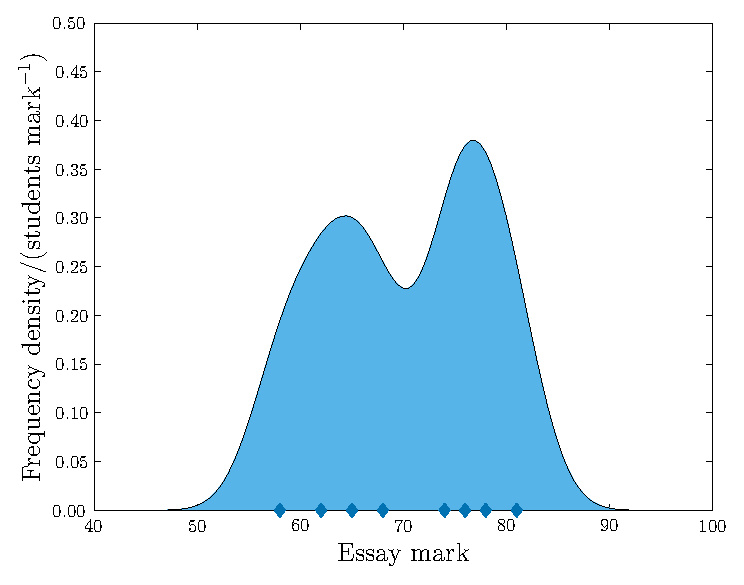
\includegraphics[width=0.47\textwidth]{./figs/Fig_2014_marks}}  
\caption{Distribution of essay marks for both cohorts of students. The diamonds indicate the actual marks; the frequency densities have been constructed by smoothing with a Gaussian kernel with a standard deviation of $\sqrt{10}~\mathrm{marks}$. The mean mark of the 2013/2014 students is $(68.1\pm3.4)~\mathrm{marks}$, and the mean for 2014/2015 students is $(70.3\pm2.7)~\mathrm{marks}$, where the uncertainties quoted on the means are estimated from the standard errors \citep[chapter 22]{Mackay2003}.}
  \label{fig:marks}
\end{figure}

Before we can draw conclusions from the distribution marks, it is necessary to consider the aptitudes of the students. Ideally, we would like to compare with marks from their first-year essays, to assess progress. I do not have access to these. However, I do have their average mark from first-year (a mark between $0$ and $100$). We would expect this to be correlated with their second-year essay mark. In \figref{diff}, we plot the distribution of differences between essay marks and their first-year averages.\footnote{Using relative difference instead of absolute difference gives qualitatively similar distributions.} We use the same Gaussian smoothing as in \figref{marks}. The 2013/2014 distribution shows a bimodal structure, with some students doing better than expected on their essay and others doing worse. The division is not related to tutorial group. There is no clear outlier (the high scoring student from \figref{2013-marks} has been absorbed into the better-than-expected peak). The 2014/2015 distribution is more consistent with expectations; the bimodality seen in \figref{marks} is an artefact of having two groups of different abilities.
\begin{figure}
  \centering
   \subfigure[{2013/2014}]{\label{fig:2013-diff} \includegraphics[width=0.47\textwidth]{./figs/Fig_2013_mark_diff}} \quad
   \subfigure[{2014/2015}]{\label{fig:2014-diif} \includegraphics[width=0.47\textwidth]{./figs/Fig_2014_mark_diff}}  
\caption{Distribution of difference between essay and average first-year marks for both cohorts of students. The diamonds indicate the actual mark differences; the frequency densities have been constructed by smoothing with a Gaussian kernel with a standard deviation of $\sqrt{10}~\mathrm{marks}$. A positive difference indicates the student did better on the essay than in first year. The mean mark difference of the 2013/2014 students is $(2.7\pm4.3)~\mathrm{marks}$, and the mean for 2014/2015 students is $(2.1\pm2.0)~\mathrm{marks}$. Averaging across both cohorts, the mean mark difference is $(2.4\pm2.3)~\mathrm{marks}$. The uncertainties quoted on the means are estimated from the standard errors.}
  \label{fig:diff}
\end{figure}

The difference between the two years is striking, but we are dealing with small sample sizes. In 2013/2014 I had one student who took special interest in the essay, and another who took no interest in revision and so underperformed in exams; the factors can go some way towards accounting for the over-performance in the essay compared to first year. Equally, I had one student who misjudged the level of rigour needed in an essay and performed worse than I expected given their enthusiasm and scientific ability.\footnote{They resubmitted and their second mark was more consistent with their first-year mark. The difference after remarking was $-5~\mathrm{marks}$ and I suspect further that improvement would have been achieved if they were not conscious of the cap at $60~\mathrm{marks}$.} In 2014/2015 I had students who achieved higher marks in first-year, it is much more difficult for them to achieve a significantly higher mark in their essays, so one might expect the differences to taper off. Without a larger population of results, we must be cautious in drawing conclusions.

While it is possible to explain away differences, this does neglect the fact that there will always be a range of student abilities and motivations. Teaching must take this diversity into account. In \figref{mark-mark-diff}, we further examine the difference between the essay and first-year marks. In 2014/2015 there is no obvious correlation between the mark difference and performance in the essay, this is not the case in 2013/2014. Those who did well seem to show significant improvement compared to first year, while those who did badly show under-performance, although the two clusters overlap in terms of essay mark. This is evidence of my 2013/2014 teaching having a polarising effect: those who were able to assimilate it went on to perform well, but those who were unable performed badly. In 2014/2015, my teaching of essay writing was more evenly distributed throughout the year (see \secref{essay-methods}), and involved a greater variety of methods; this may have made it more accessible and easier to digest, benefiting a greater selection of students. However, in distributing the teaching, it seems to have lost some of its impact, and there is not as great an increase in marks. Moving some of the discussion to the Autumn term, may have diluted the impact of giving advice while the essay was being written. It appears that there are potentially advantages and disadvantages to the adaptations I made to my teaching schedule.
\begin{figure}
  \centering
   \includegraphics[width=0.6\textwidth]{./figs/Fig_mark_mark_diff}
\caption{Difference between essay and average first-year marks as a function of essay marks. The red--orange squares are the results for the 2013/2014 students and the light blue circles are for the 2014/2015 students. The 2013/2014 appear to fall into two clusters: those with positive mark differences and those with negative mark differences. The mean essay mark for the positive-difference group is $(73.3\pm4.5)~\mathrm{marks}$, and the mean for the negative-difference group is $(61.3\pm1.4)~\mathrm{marks}$, where the uncertainties quoted are estimated from the standard errors.}
  \label{fig:mark-mark-diff}
\end{figure}

There is one further statistic that can be incorporated into our analysis, tutorial attendance. We would expect attendance to be correlated with attainment. First, there is a causal link: those who spend more time engaging with educational activities should see a greater benefit from them. Second, attendance can be linked to motivation, which is correlated with learning \citep[e.g.,][chapter 4]{Ramsden1992}. Absence from tutorial could be because of apathy or disorganisation (see \secref{other-discuss}); because of poor health or personal matters, or because a clash with another educational activity such as an extracurricular or careers event. The first set of reasons indicates a lack of engagement with or low-prioritisation of their studies, which would be correlated with poor attainment. The second set does indicate anything about how the student views the subject or their studies, but may still be linked to a lack of motivation as a side effect of potentially depressing problems. The final set may indicate that the student is positively engaged in their studies, taking an active interest in the subject or their own achievement; this may indicate good attainment if this benefit outweighs the disadvantage of missing teaching sessions. In \figref{attend} we plot fractional attendance for year (the $20$ tutorials) against essay mark. There is no obvious correlation for 2013/2014, but there does appear to be the expected positive trend for 2014/2015.
\begin{figure}
  \centering
   \includegraphics[width=0.6\textwidth]{./figs/Fig_attend}
\caption{Essay mark as a function of tutorial attendance. The red--orange squares are the results for the 2013/2014 students and the light blue circles are for the 2014/2015 students. There are $20$ tutorials, hence attendance is quantized into divisions on $0.05$.}
  \label{fig:attend}
\end{figure}

The difference between the cohorts could again be attributed to the small sample sizes; however, it may also trace the difference in teaching. In 2013/2014, teaching of essay writing was concentrated to tutorials 12 and 14 (see \tabref{2013-14}). Attendance at these two sessions was perfect. Hence no students suffered from missing an important lesson. The second-order effect of the impact of motivation (as traced by attendance) on performance appears to be negligible. In 2014/2015, teaching of communication skill was distributed throughout the year, making any given absence more significant. If we only consider the main essay-writing tutorials 3, 12, 13 and 14 (\tabref{2014-15}), the trend persists.  One student attended half of these tutorials and received an essay mark of $62~\mathrm{marks}$; two attended three out of four and received a mean mark of $(67.0\pm6.4)~\mathrm{marks}$, and the remaining five attended all four and have an mean mark of $(73.2\pm2.7)~\mathrm{marks}$. The quoted uncertainties on the means have been estimated from the standard error \citep[chapter 22]{Mackay2003}. Attendance appears to correlate with performance as being absent from tutorial means that students miss useful teaching. The provision of written materials, like a blog (\secref{blog}), that can be studied any time may ameliorate the impact of missing tutorial, but only if students are aware of their existence and importance. Breaking up teaching across multiple tutorials increases the probability that one or more sessions will be missed; however, it also reduces the probability that all of the teaching on essay writing is missed, which would likely be extremely detrimental.

\section{Summary \& conclusion}\label{sec:marks-end}

From the limited data available, we may draw some provisional qualitative conclusions on the effectiveness of teaching. Making more robust statements would require a more sophisticated analysis or further data. Unsurprisingly, our data suggest that essay-writing ability is correlated both with overall proficiency (measured by average first-year mark) and attendance at tutorials where essay writing was discussed. Comparing the two cohorts, it appears that the more distributed teaching of 2014/2015 is safer. Students are less likely to under-perform and there is a lower risk of missing all the relevant teaching. However, the teaching of 2013/2014 was more effective at inspiring significant over-performance (compared to the first-year mark). This may be because a concentrated session during the Spring term is particularly effective, as students can immediately make use of the information, but we do not have the evidence to prove this. We conclude, that neither the teaching of 2013/2014 nor 2014/2015 is superior to the other in all regards.


\backmatter

\phantomsection
\bookmarksetup{startatroot}

\bibliographystyle{../physicsAuthorYearURL2}
\addcontentsline{toc}{chapter}{References}
\bibliography{../teaching}

\end{document}
